\documentclass{tesis-usb}

% paquetes
\usepackage[utf8]{inputenc}
\usepackage{verbatim}
\usepackage{acronym}
\usepackage{amsmath}
\usepackage{amsfonts}
\usepackage{amssymb}
\usepackage{makecell}
%\usepackage{hyperref}

% Para los graficos al final...
\usepackage{float}
\usepackage{placeins}

% Para arreglar espacio entre parrafos y sangria
\usepackage{parskip}
\setlength{\parindent}{3ex}

% workaround
\DeclareMathSymbol{.}{\mathord}{letters}{"3B}

% plot
\usepackage{pgfplots}
\usetikzlibrary{pgfplots.statistics}

% fragmentos de código
\usepackage{listings}
\renewcommand{\lstlistingname}{Fragmento de Código}
\renewcommand{\lstlistlistingname}{Índice de Fragmentos de Código}
\lstset{
	basicstyle=\ttfamily\footnotesize,
	frame=single,
	captionpos=b,
	numbers=left,
	showstringspaces=false,
	aboveskip=1em,
	belowskip=2em,
	xleftmargin=1em,
	xrightmargin=1em,
	tabsize=4}

% estilo de las referencias
\usepackage[fixlanguage]{babelbib-and}\selectbiblanguage{spanish}
\usepackage{url}
%\bibliographystyle{babplain-lf}
\bibliographystyle{babunsrt-lf}


\autor{Christhian Guevara Valencia}
\autori{C. Guevara}
\usbid{09-10381}
\titulo{Sistema de Recomendación de Soluciones a Errores de Programación en Lenguaje C usando Minería de Datos}
\fecha{Noviembre~de~2018}
\agno{2018}
\fechadefensa{10~de~Diciembre~de~2018}
\tutor{Ph.D. Masun Nabhan Homsi}
% \usarcotutor
\cotutor{Nombre y Apellido \mbox{(Afiliaci\'on)}} 
\trabajo{Proyecto de Grado}
\coord{Ingeniería de la Computación}
\grado{Ingeniero de Computación}
\carrera{Ing. Computación}
\programa{Nombre del Programa}
\juradouno{Nombre y Apellido}
\juradodos{Nombre y Apellido \mbox{(Afiliaci\'on)}}
\juradotres{Nombre y Apellido}

\begin{document}

\frontmatter
\maketitle
\newpage
\thispagestyle{empty}
\vspace*{-3.4cm}
\hspace*{-1cm}
\makebox[\textwidth]{

\includegraphics[width=\paperwidth]{img/img00.jpg}
}
\newpage
\thispagestyle{empty}
\vspace*{-3.4cm}
\hspace*{-1cm}
\makebox[\textwidth]{

\includegraphics[width=\paperwidth]{img/img01.jpg}
}
\begin{resumen}
En los \'ultimos a\~nos ha crecido la popularidad de los sitios de preguntas y respuestas como un recurso informativo,
capaz de proveer a sus usuarios de un medio para obtener soluciones a diversos problemas.
Se sabe que los programadores tienden a invertir gran parte de su tiempo buscando soluciones a errores en estos sitios.
%invirtiendo incluso un 19\% del tiempo que disponen.

Asimismo, estudios previos han demostrado la baja efectividad de ciertos
motores de b\'usqueda al emplear c\'odigo en sus consultas, entre ellos Stack Overflow.
Lo que fuerza al programador a intentar describir su problema en breves l\'ineas
y dificulta la b\'usqueda de informaci\'on. 

Surge la necesidad de desarrollar una herramienta que automatice el proceso,
por tal motivo se desarroll\'o un Sistema de Recomendaci\'on para ayudar al programador a identificar errores mediante sugerencias,
que emplea fragmentos de c\'odigo para la consulta y 
aplica algoritmos de Miner\'ia de Datos para explotar los conocimientos de la comunidad de usuarios de Stack Overflow.

Se compararon las fortalezas y debilidades de las t\'ecnicas de similitud entre documentos
y se decidi\'o usar una modificaci\'on del esquema de Document Fingerprinting,
que emplea la t\'ecnica de MinHash para realizar comparaciones entre fragmentos de c\'odigo
y utiliza la t\'ecnica de Locality-Sensitive Hashing para indexar los fragmentos.

Las pruebas realizadas sobre el \'indice mostraron una efectividad del 100\%
sobre una muestra de $1.000$ fragmentos de c\'odigo extra\'idos de los t\'opicos.
Al emplear otra muestra de 10 fragmentos extra\'idos de fuentes externas mostr\'o ser eficaz al 60\%,
sugiriendo t\'opicos relacionados. Se concluye entonces que el sistema
implementado cumple cabalmente la funci\'on para la cual fue dise\~nado.

\vfill
\textbf{Palabras clave:} MinHash, LSH, Sistema de Recomendación, Stack Overflow, Plugin para Eclipse.
\end{resumen}
\chapter*{Dedicatoria}

A mi madre, quien me ha dado todo cuanto ha podido y
a mi padre, cuya alegría no tendría fin.
\chapter*{Agradecimientos}

A la Profa. Masun Nabhan Homsi, por la gran paciencia que me brindó a lo largo de la
elaboración de este Proyecto de Grado, sin ella no habría sido posible.

A mi abuela y a mis familiares,
por tener la dicha de estar con personas como ustedes,
en las buenas y malas me han brindado su apoyo.
\tableofcontents
\listoftables
\listoffigures
\lstlistoflistings
\useacronyms

\mainmatter
% Para la sangría
\chapter*{Introducción}

Desarrollar software es una actividad en constante evolución,
que con frecuencia obliga al programador a enfrentarse a nuevos desafíos,
debido a la creciente complejidad de los sistemas modernos.

Gran parte de estos desafios consiste en solucionar errores inesperados,
que surgen espontáneamente en la mayoría de los proyectos de software.
Estos fallos, denominados \textit{bugs}, se originan debido a errores de lógica o comprensión,
e incluso por comportamientos no definidos o inesperados~\cite{monperrus:hal-00987395}.
Su solución se dificulta al toparse con documentación escasa, incomprensible o inexistente.

Estudios muestran que el programador invierte hasta un 19\% de su tiempo~\cite{Brandt:2009:TSO:1518701.1518944}
consultando diversas fuentes~\cite{Ko:2007:INC:1248820.1248867},
entre las que destacan los recursos en línea~\cite{10.1007/978-0-387-09684-1_21}.

Los recursos en línea disponibles son variados y amplios,
siendo notables: Los foros, los blogs, las listas de correo electrónico, entre otros.
En particular, los sitios de preguntas y respuestas \ac{QA},
como \textit{Stack Overflow}, cuyos tópicos se enfocan en 
la resolución de problemas de programación
y conforman un conjunto aprovechable de conocimientos de libre acceso.

Sin embargo, surgen problemas inherentes al proceso de búsqueda,
entre los cuales destaca la falta de automatización~\cite{Ponzanelli:2014:PSR:2705615.2706035}.
Saber qué y cómo buscar información no es trivial,
el programador debe tener cierto grado de habilidad para realizar
búsquedas cuyos resultados sean satisfactorios~\cite{Stolee:2014:SSS:2628068.2581377}.

Por otro lado, las consultas hechas por los programadores
suelen emplear palabras clave que no se relacionan directamente con el código fuente.
El motivo aparente es la ineficacia de algunos motores de búsqueda para realizar este tipo de consultas,
un caso notable es el motor de búsqueda del sitio web de \textit{Stack Overflow}~\cite{monperrus:hal-00987395}.

\section*{Planteamiento del Problema}
La corrección de errores en el software es un proceso repetitivo y sistemático,
que puede llegar a ser tedioso y frustrante para el programador.
En general, tratar de resolver errores requiere consultar múltiples fuentes con frecuencia,
para buscar información que ayude a solucionar el error,
existiendo la posibilidad de no encontrar información adecuada.

Al programador no le es posible utilizar los motores de búsqueda para consultar el código directamente,
sino que, por el contrario, tiende a describir su problema brevemente enfatizando los puntos clave;
entre ellos, se incluye el nombre de la función, la clase, la librería o paquete,
los resultados obtenidos por el program, los errores indicados por el compilador,
la funcionalidad implementada, entre otros. En cualquier caso,
debe ser lo suficientemente perspicaz para describir correctamente el problema e identificar su origen.

Usualmente el programador tiende a consultar la documentación en busca de la solución al problema,
solo para encontrarse con que la documentación no abarca los conceptos necesarios para su resolución;
también, es posible que la misma sea de difícil comprensión para el programador,
al estar escrita de forma confusa, con términos complejos o en otro idioma;
además, cabe la posibilidad de que esté desactualizada y 
las características asociadas al problema estén relacionadas con una nueva implementación,
aún sin documentar o en el peor de los casos, no exista.
Lo que con seguridad impide al programador encontrar la solución al problema en periodos razonables de tiempo;
en el peor de los casos, puede obstaculizar y posponer la realización de la tarea asignada.

El programador que no ha encontrado la solución en la documentación,
con frecuencia recurre a otros sitios, entre ellos se encuentran los sitios de preguntas y respuestas.
Estos sitios permiten al usuario consultar a otros usuarios sobre el problema presentado,
permitiendo que las personas que hayan pasado por una situación similar
o con un conocimiento más amplio, respondan.
Estas respuestas quedan registradas en el foro y sirven como retroalimentación,
para el uso posterior por parte de otros usuarios.

Sin embargo, éste proceso es lento y requiere la intervención de otros usuarios.
Además, parte de las preguntas hechas por los usuarios se repite periódicamente,
a pesar que se enfatiza e insta a los usuarios a realizar una búsqueda anticipada.
Lo que se debe en esencia, a la falta de habilidad de algunos usuarios para realizar
consultas cuyos resultados sean satisfactorios.

\section*{Antecedentes}

Trabajos previos en el área apuntan a desarrollar un Sistema de Recomendación
que se beneficie del conocimiento provisto por la comunidad de \textit{Stack Overflow},
cuya principal motivación es proveer herramientas al usuario que agilicen el proceso de búsqueda.

Se han publicado diversas investigaciones en éste sentido, entre las que destacan:

\begin{itemize}
	\item \textbf{Debugging with the Crowd}\cite{monperrus:hal-00987395}
	presenta un Sistema de Recomendación como una herramienta para \textit{debugging}.
	Realiza un estudio empírico sobre la base de datos de Stack Overflow y establece las bases
	para el desarrollo de un sistema de recomendación que emplee los conocimientos de la comunidad de usuarios.
	
	\item \textbf{Prompter}\cite{Ponzanelli:2014:PSR:2705615.2706035} es un Sistema de Recomendación
	basado en \textit{Stack Overflow} que se muestra como un \textit{plug-in} para \textit{Eclipse},
	presenta un modelo de clasificación basado en las características del código y el contexto en
	el \textit{IDE}.

	\item \textbf{PDE4Java}\cite{Jadalla:2008:PPD:1413814.1413815} es un motor 
	para la detección de plagio en código fuente para \textit{Java}, indaga en
	las bases del uso del \textit{MinHash} como una potente herramienta.
\end{itemize}

Gran parte de la literatura relacionada, se enfoca en el estudio de distintas técnicas
que abordan el problema de encontrar similitudes en el código.

\section*{Justificación}

El presente Proyecto de Grado se aboca en el desarrollo e implementación de 
un Sistema de Recomendación, con la finalidad de proveer sugerencias 
relevantes al programador.

Muchos de los problemas que afectan el desarrollo de software se relacionan
directamente con el proceso de búsqueda de información. El programador
invierte tiempo valioso y sus consultas pueden no ser exitosas.
Incrementando la brecha entre los objetivos y el resultado.

Queda en evidencia la falta de herramientas
que faciliten el proceso de búsqueda al desarrollador,
permitan realizar consultas relacionadas con el código
y disminuyan el tiempo empleado.

Parte del enfoque de este Proyecto consiste en aplicar un algoritmo
eficaz que permita reconocer fragmentos de código estructuralmente similares,
salvando la gran cantidad de diferencias que pueden presentarse.

\section*{Objetivos}

\subsection*{Objetivo General}

%Desarrollar un Sistema de Recomendación capaz de sugerir tópicos en el sitio web
%de \textit{Stack Overflow} que sean de relevancia para el programador,
%ayuden a solucionar errores y agilicen el proceso de desarrollo de software
%en el lenguaje c/c++, apoyándose sobre algoritmos de Minería de Datos.

Desarrollar un sistema capaz de recomendar soluciones a errores cometidos por el programador en lenguaje C,
apoyándose sobre algoritmos de Minería de Datos.

\subsection*{Objetivos Específicos}
\begin{itemize}
  \item Aplicar algoritmos de minería de datos para explotar los conocimientos
  de programación en lenguaje c de la comunidad de programadores del sitio web \textit{Stack Overflow}.
  
  \item Implementar una herramienta que ayude al programador a identificar errores en el código,
  mediante una lista de recomendaciones de posibles soluciones proporcionada por la comunidad.

  \item Establecer un modelo de clasificación que incluya aspectos relacionados
  a la reputación de los usuarios de \textit{Stack Overflow}.
\end{itemize}

\section*{Organización del Libro}
El presente Proyecto de Grado está estructurado en cuatro capítulos.
En el Capítulo 1, el marco teórico,
se presentan los planteamientos necesarios para la comprensión del desarrollo del Sistema de Recomendación.
En el Capítulo 2, el marco tecnológico,
se exponen las herramientas empleadas que permitieron la implementación del Sistema de Recomendación.
En el Capítulo 3, el marco metodológico,
se desglosan los procesos, métodos y técnicas aplicadas para la elaboración del Sistema de Recomendación.
En el Capítulo 4, desarrollo y resultados,
se describen los resultados obtenidos al emplear el índice invertido e implementar el Sistema de Recomendación.

\chapter{Marco Teórico}

En este capítulo se definen los conceptos necesarios para la comprensión
del Sistema de Recomendación del presente Proyecto de Grado.
En primer lugar, en la Sección \ref{sec:min}, se provee una breve introducción a Minería de Datos.
En segundo lugar, en la Sección \ref{sec:sr}, se presentan los fundamentos de un Sistema de Recomendación.
En tercer lugar, en la Sección \ref{sec:qa}, se describen los Sitios de Preguntas y Respuestas.
En cuarto lugar, en la Sección \ref{sec:sim}, se expone la Similitud entre Documentos como un área de investigación.
Posteriormente, en la Sección \ref{sec:doc}, se detalla la técnica de \textit{Document Fingerprinting} empleada.
Finalmente, en la Sección \ref{sec:ind}, se enuncian las bases para la elaboración del Índice Invertido.

\section{Minería de datos}
\label{sec:min}

“La Minería de Datos \dots~implica la deducción de algoritmos que exploran los datos,
desarrollan el modelo y descubren patrones previamente desconocidos”~\cite{Maimon:2010:DMK:1869923}.

El objetivo general del proceso de minería de datos consiste en extraer
información de una fuente de datos e intentar convertir esa información
en un conjunto aprovechable de conocimientos.

El proceso de minería de datos generalmente consiste de 3 pasos~\cite{Amatriain2011}:

\begin{itemize}
  \item Preprocesamiento.
  \item Análisis.
  \item Interpretación.
\end{itemize}

Los Sistemas de Recomendación nacen como consecuencia de automatizar el
proceso de una técnica de minería de datos, para una instancia en particular.
 
\section{Sistema de Recomendación}
\label{sec:sr}

Los Sistemas de Recomendación son agentes de software que obtienen los intereses
o preferencias de los usuarios, para hacer las recomendaciones correspondientes~\cite{Xiao:2007:EPR:2017327.2017335}.
Generalmente, éstas sugerencias se generan utilizando información perteneciente al usuario,
ya sea que esta información fuere adquirida de forma explícita o implícita.

\subsection{Objetivos}

El objetivo principal de un Sistema de Recomendación es realizar sugerencias 
que permitan agilizar un proceso.

Además, se mencionan los siguientes objetivos operacionales y técnicos~\cite{Aggarwal2016}:

\begin{description}
  \item [Relevancia] Recomendar elementos que sean relevantes para el usuario es el objetivo operativo esencial de un Sistema de Recomendación.
  \item [Novedad] Si el contenido del tópico recomendado es diferente a los que ha visto el usuario en el pasado pero sigue siendo útil.
  \item [Serendipia] Los elementos recomendados son algo inesperados y por lo tanto, hay un modesto sentimiento de descubrimiento afortunado, en contraposición a las recomendaciones obvias.
\end{description}

\subsection{Modelos Básicos}

Se definen tres modelos básicos de Sistemas de Recomendación~\cite{jannach_zanker_felfernig_friedrich_2010}:

\subsubsection{Filtrado Colaborativo}

Los Sistemas de Recomendación que utilizan modelos de filtrado colaborativos
realizan sus recomendaciones empleando las calificaciones proporcionadas por múltiples usuarios.
La idea básica consiste en totalizar las calificaciones sobre los elementos,
reconocer aquellas calificaciones que son comunes entre los usuarios y
generar nuevas recomendaciones basadas en la comparación de estas calificaciones.
En otras palabras, aprovechar las correlaciones entre elementos o
las correlaciones entre los usuarios para el proceso de predicción.

\subsubsection{Basados en Contenido}

En los Sistemas de Recomendación basados en contenido,
los atributos descriptivos de los elementos se usan para hacer recomendaciones,
el término contenido se refiere a estos atributos.
Se establecen perfiles para los elementos,
se encuentran aquellos que comparten características similares y
se recomiendan a los usuarios en base a elecciones anteriores.

\subsubsection{Basados en Conocimiento}

En los Sistemas de Recomendación basados en conocimiento,
las recomendaciones se llevan a cabo en base a las similitudes
entre los requerimientos del usuario y las características de los elementos.
Durante el proceso de recuperación se utilizan diversas reglas y
funciones de similitud provenientes del uso de bases de conocimiento.
Este enfoque toma su nombre de las bases de conocimiento.

\subsubsection{Sistemas Híbridos}

Los modelos básicos de Sistemas de Recomendación, explotan diferentes fuentes de datos.
Los sistemas híbridos pueden combinar las fortalezas de varios tipos
de Sistemas de Recomendación para crear un modelo más robusto;
además de combinar múltiples fuentes de datos,
también pueden mejorar la eficiencia de una clase en particular.

\section{Sitio de Preguntas y Respuestas}
\label{sec:qa}

Un \ac{QA} o sitio de preguntas y respuestas,
permite a sus usuarios adquirir, compartir y generar
conocimiento al interactuar con la comunidad.
%Los usuarios pueden consultar, participar y contribuir
%activamente con la comunidad a través de internet.

Se compone de tres partes fundamentales:

\begin{description}
  \item [Preguntas] Las preguntas son formuladas por los usuarios para describir
  un problema con el fin de obtener una solución por parte de la comunidad.
  %Es necesario que el usuario recolecté toda la información necesaria al momento de formular la pregunta.
  \item [Respuestas] Las respuestas son suministradas por otros usuarios y %supondrán una contribución a la comunidad como 
  representan posibles soluciones al problema planteado en la pregunta asociada.
  %Es posible que varias de estas posibles soluciones puedan resolver el problema.
  \item [Comentarios] Los comentarios son utilizados por los usuarios para agilizar el proceso; 
  permiten aclarar detalles, sugerir correcciones o proveer información.
\end{description}

\subsection{Stack Overflow}

\textit{Stack Overflow} es un \ac{QA} perteneciente a la red \textit{Stack Exchange},
que se enfoca en la resolución de problemas de programación.

El contenido de los tópicos es provisto por la comunidad y
conforma un conjunto aprovechable de conocimientos de libre acceso.

\subsubsection{Estructura de la Base de Datos}
\label{subsec:EstBasDat}

La base de datos de \textit{Stack Overflow} se compone de 8 tablas distintas,
cuya descripción se presenta a continuación:

\begin{description}
  \item [Badges] Conjunto que comprende a las medallas otorgadas a cada usuario.
  Son premios por contribuir activamente con la comunidad.
  \item [Comments] Conjunto que comprende a los comentarios asociados a los tópicos.
  Permite agilizar el intercambio de información.
  \item [PostHistory] Conjunto que comprende cada una de las modificaciones realizadas a los tópicos.
  Un historial de cambios.
  \item [PostLinks] Conjunto que comprende a los enlaces entre tópicos,
  ya sean tópicos relacionados o tópicos duplicados.
  \item [Posts] Conjunto que comprende el contenido esencial del sitio, los tópicos;
  ya sean éstos preguntas o respuestas.
  \item [Tags] Conjunto que comprende a todas las etiquetas que han sido asociadas a los tópicos.
  Cada tópico puede tener hasta 5 etiquetas asociadas.
  \item [Users] Perfil del usuario, conjunto que comprende la información pública para cada usuario.
  \item [Votes] Reputación de los tópicos, conjunto que comprende cada voto asignado a los tópicos.
\end{description}

Se puede encontrar el diagrama \textit{entidad-relación} en el Anexo \ref{ape:diag},
así como una descripción detallada del contenido de las tablas.
%Además, se incluyen un enlace al diagrama general de la base
%de datos de los sitios web pertenecientes a la red \textit{Stack Exchange}.

\section{Similitud entre Documentos}
\label{sec:sim}

Existen diversas áreas de investigación que abordan el problema de encontrar
documentos similares, entre ellas se encuentran Detección de Plagio
y Detección de Clones.

\subsection{Detección de Plagio}
\label{subsec:plagio}

“Plagio, es el acto de tomar los escritos de otra persona y pasarlos como propios.
El fraude está estrechamente relacionado con la falsificación y la piratería,
prácticas generalmente en violación de las leyes de derechos de autor”~\cite{britannica_2017}.

Las características propias de los lenguajes de programación,
se presentan como dificultades para el análisis de similitud textual~\cite{Beth2014ACO},
permitiendo realizar una gran cantidad de cambios al código.

A continuación, se enumeran los modificaciones más comunes~\cite{Arwin:2006:PDA:1151699.1151730}:

\begin{itemize}
  \item cambio de formato
  \item cambio de identificadores
  \item cambio en el orden de los operandos en las expresiones
  \item cambio del tipo de datos
  \item sustitución de expresiones por sus equivalentes
  \item introducción de declaraciones redundantes
  \item cambio en el orden de declaraciones independientes del tiempo
  \item cambio en la estructura de las instrucciones de iteración
  \item cambio en la estructura de las declaraciones de selección
  \item sustitución de las llamadas a función por el cuerpo de la misma
  \item introducción de declaraciones no estructuradas
  \item combinación de fragmentos de código originales y copiados
  \item traducción del código fuente de un lenguaje a otro
\end{itemize}

\newpage
El plagio generalmente ocurre en dos niveles~\cite{Aggarwal2016}:

\begin{description}
  \item [Plagio Textual] El documento plagiado es idéntico o similar al documento original, el cual puede ser un informe, un ensayo, un reporte, entre otros.
  \item [Plagio de Código Fuente] El código plagiado es una copia completa o parcial del código original, que ha sido adulterado para pasarlo como propio.
\end{description}

\subsection{Detección de Clones}
\label{subsec:plagio}
Un clon es un fragmento de código que ha sido copiado,
aún si éste ha sufrido modificaciones menores
o ha sido adaptado a otro contexto.
Sin embargo, su definición es vaga y muchas veces depende de los algoritmos
y los ajustes utilizados~\cite{Roy07asurvey}.

Aunque los enfoques son distintos,
tanto el área de Detección de Clones,
como el área de Detección de Plagio en Código Fuente,
se fundamentan en determinar la similitud entre fragmentos de código arbitrario~\cite{Beth2014ACO}.

A continuación, se presenta una clasificación de los tipos de clones
basada en el tipo de similitud~\cite{Roy07asurvey}:

\begin{description}
  \item [Tipo I] Fragmentos de código idénticos exceptuando las variaciones en los espacios en blanco, el diseño y los comentarios.
  \item [Tipo II] Fragmentos de código sintácticamente idénticos exceptuando las variaciones en los identificadores, los literales, los tipos, el diseño y los comentarios.
  \item [Tipo III] Fragmentos de código con modificaciones adicionales. Las expresiones pueden estar alteradas y tener variaciones en los identificadores, los literales, los tipos, el diseño y los comentarios.
  \item [Tipo IV] Fragmentos de código que realizan el mismo cálculo pero implementados a través de diferentes variantes sintácticas.
\end{description}

\newpage
\subsection{Métodos y Técnicas}

Numerosos métodos y técnicas han sido desarrollados para abordar
el problema de similitud entre fragmentos de código.

Una clasificación general fundamentada en el tipo de comparación es provista~\cite{Roy07asurvey}:

\begin{description}
  \item [Comparación basada en texto] Busca coincidencias textuales exactas entre segmentos; por ejemplo, ejecuciones de cinco palabras. De ejección rápida, pero puede confundirse al renombrar identificadores.
  \item [Comparación basada en lexemas] Similar a la comparación textual, pero usando un \textit{lexer} para convertir el programa en \textit{tokens}. Se descartan los espacios en blanco, los comentarios y los nombres de los identificadores.
  \item [Comparación basada en árboles de sintaxis] Se construyen y comparan los árboles de sintaxis abstracta, permitiendo detectar similitudes de mayor nivel; por ejemplo, puede normalizar sentencias condicionales y detectar constructos equivalentes.
  \item [Comparación basada en grafos de dependencia] Captura el flujo de control en un programa y permite ubicar equivalencias de niveles mucho más altos, que involucra una mayor complejidad y tiempo de cálculo.
  \item [Comparación basada en métricas] Calculan puntajes para segmentos de código de acuerdo a ciertos criterios; por ejemplo, el número de ciclos y condicionales. Sin embargo, puede dar lugar a falsos positivos.
  \item [Comparación empleando enfoques híbridos] Por ejemplo, árboles de sintaxis abstracta con árboles de sufijo, puede combinar la capacidad de detección de árboles de sintaxis abstracta con la velocidad que permiten los árboles de sufijo.
\end{description}

\section{Document Fingerprinting}
\label{sec:doc}

Es una técnica para la detección precisa de copias completas 
y parciales entre documentos~\cite{Lindkvist2005WinnowingA}.
El texto se divide en subsecuencias, se calcula el \textit{hash} para cada 
subsecuencia y se comparan los valores de \textit{hash} obtenidos entre los documentos. 
Este proceso se realiza con la idea de que la reducción de la dimensionalidad resultante,
supondrá una comparación mucho más factible y conservará la misma relación de similitud.
En otras palabras, si un valor \textit{hash} es igual a otro valor \textit{hash}, 
es muy probable que los textos correspondientes también sean idénticos~\cite{Beth2014ACO}.

\subsection{Subsecuencias}

El texto se divide en subsecuencias mediante el uso de \textit{n-gram} o \textit{w-shingling},
donde el $n$ y el $w$ son parámetros escogidos por el usuario~\cite{Beth2014ACO}.

\subsubsection{N-Grams}

Un \textit{n-gram} es una subsecuencia de $n$ elementos contiguos,
creada a partir de una secuencia dada. Por ejemplo, 
la secuencia de \textit{4-grams} de la siguiente frase
‘pablito clavó un clavito’ es:

\begin{equation*}
pabl\ abli\ blit\ lito\ itoc\ toca\ ocav\ cavo\ avou\ voun\ ounc\ uncl\ ncla\ clav\ lavi\ avit\ vito
\end{equation*}

\subsubsection{W-Shingles}

Un \textit{shingle} es una subsecuencia contigua de palabras. 
Por su parte, una subsecuencia contigua de $w$ palabras es un \textit{w-shingle}.
Por ejemplo, el conjunto de \textit{2-shingles} de la frase ‘compré pocas copas, pocas copas compré’ es:

\begin{equation*}
(compre,\ pocas),\ (pocas,\ copas),\ (copas,\ pocas),\ (copas,\ compre)
\end{equation*}

\subsubsection{Hashing}

Las subsecuencias de texto obtenidas mediante \textit{n-grams}
o \textit{w-shingles} no suelen usarse directamente;
por el contrario, se escoge una función de \textit{hash} que convierte cada una de las
subsecuencias de texto a una representación numérica.

Por ejemplo, se podría escoger una representación de \textit{n-grams} de $n = 7$
para un documento; luego, se utiliza una función de \textit{hash} y 
se convierten los \textit{7-grams} a una representación numérica
en el rango de $0$ a $2^{32} - 1$. 
En consecuencia, cada \textit{7-gram} es representado por \textit{4 bytes} en vez de \textit{7 bytes},
lo que compacta el tamaño de los datos y permite realizar operaciones sobre enteros.

\subsection{Similitud}

%La medida de similitud entre documentos se puede derivar del número de las partes compartidas entre los documentos.
Si se ve al documento como un conjunto, los elementos del conjunto serán aquellos valores de \textit{hash} que son calculados a partir del documento.
De esta manera, los documentos que compartan fragmentos de texto similares tendrán elementos comunes en sus conjuntos,
incluso si estos fragmentos aparecen en diferente orden en los documentos~\cite{Rajaraman:2011:MMD:2124405}.

\subsubsection{Coeficiente de Similitud de Jaccard}

Se mide la similitud de conjuntos por el coeficiente de similitud de \textit{Jaccard},
el cual para los conjuntos $A$ y $B$ es~\cite{Rajaraman:2011:MMD:2124405}:

\begin{equation*}
J(A, B) = \frac{|A \cap B|}{|A \cup B|}
\end{equation*}

Esto es, la relación entre el tamaño de la intersección de $A$ y $B$ con el tamaño de su unión.
El valor obtenido se encuentra entre $0$ y $1$, 
siendo $1$ cuando los conjuntos son iguales y 
$0$ cuando son diferentes. 
Los valores intermedios definen el grado de similitud.

\subsection{Huella Digital}

La técnica de \textit{Document Fingerprinting} no se limita a 
comparar los valores de \textit{hash} obtenidos de los documentos directamente; 
en su lugar, se selecciona un subconjunto de estos valores de \textit{hash}
para crear el \textit{fingerprint} o huella digital.
De esta manera, se puede representar el documento en menos espacio
y realizar comparaciones mucho más rápidas.

\subsubsection{Firma}

La mayoría de las técnicas utilizadas en \textit{Document Fingerprinting} 
son diseñadas para detectar diferencias entre documentos,
generando valores de \textit{hash} que difieren significativamente si hay cambios.
En contraposición, se utiliza una firma para detectar similitudes entre documentos,
produciendo valores de \textit{hash} similares para documentos similares.

\subsubsection{MinHash}

El \textit{MinHash} está diseñado con el fin de que dos objetos
similares generen valores de \textit{hash} similares~\cite{grattan_2017}.
Se suele utilizar ésta representación para estimar de forma eficiente
el coeficiente de similitud de \textit{Jaccard}~\cite{Rajaraman:2011:MMD:2124405}.

Una forma de visualizar el funcionamiento del método
consiste en utilizar una matriz característica,
donde las columnas corresponden a los conjuntos y
las filas a sus elementos.
De esta forma, se obtiene una matriz que contiene un $1$ en la fila $f$ y la columna $c$,
si el elemento de la fila $f$ es miembro del conjunto de la columna $c$;
caso contrario, el valor en la posición $(f,c)$ es $0$.

Luego, al escoger una permutación de las filas de la matriz, 
se tiene que el valor \textit{MinHash} para el conjunto de la columna $c$,
es el valor del elemento de la primera fila $f$ en ese orden,
para el cual el valor en la posición $(f,c)$ es $1$.

Por ejemplo, si se tiene la matriz característica cuyas filas son los elementos
$\{a,b,c,d,e\}$ y sus columnas son los subconjuntos $S_1 = \{a,d\}$,
$S_2 = \{c\}$, $S_3 = \{b,d,e\}$ y $S_4 = \{a,c,d\}$, se obtendrá la Tabla \ref{tab:conjuntoejemplo1}.

\begin{table}[h]
\caption{Matriz característica.}
\label{tab:conjuntoejemplo1}
\small
\centering
\begin{tabular}{ccccc}
\hline
{Elemento} & {$S_1$} & {$S_2$} & {$S_3$} & {$S_4$} \\
\hline
a & 1 & 0 & 0 & 1 \\
b & 0 & 0 & 1 & 0 \\
c & 0 & 1 & 0 & 1 \\
d & 1 & 0 & 1 & 1 \\
e & 0 & 0 & 1 & 0 \\
\hline
\end{tabular}
\end{table}

Luego, al generar una permutación de las filas de la matriz en la Tabla \ref{tab:conjuntoejemplo1},
tal que el orden de las filas sea ‘beadc’, se obtendrá la matriz característica
que se muestra en la Tabla \ref{tab:conjuntoejemplo2}.

\begin{table}[h]
\caption{Matriz característica permutada.}
\label{tab:conjuntoejemplo2}
\small
\centering
\begin{tabular}{ccccc}
\hline
{Elemento} & {$S_1$} & {$S_2$} & {$S_3$} & {$S_4$} \\
\hline
b & 0 & 0 & 1 & 0 \\
e & 0 & 0 & 1 & 0 \\
a & 1 & 0 & 0 & 1 \\
d & 1 & 0 & 1 & 1 \\
c & 0 & 1 & 0 & 1 \\
\hline
\end{tabular}
\end{table}

Esta permutación define una función  $h_1(x)$,
que convierte los subconjuntos $S_1, S_2, \ldots, S_n$ a filas 
$h_1(S_1), h_1(S_2), \ldots, h_1(S_n)$.
De esta forma, se obtiene el valor de \textit{MinHash} para $S_1$ de acuerdo a $h_1(x)$.
Así se tiene que, el valor del elemento de la primera fila,
que contiene un $1$ para el conjunto de la columna $S_1$ es $a$,
luego $h_1(S_1) = a$. Se obtienen los valores para $S_2$, $S_3$ y $S_4$ de forma similar,
tal que $h_1(S_2) = c$, $h_1(S_3) = b$ y $h_1(S_4) = a$.

A continuación, se escogen $2$ permutaciones distintas de las filas,
tal que el orden de las filas sea ‘cdaeb’ y ‘dbcea’, lo que genera $h_2(x)$ y $h_3(x)$,
como se muestra en la Tabla \ref{tab:conjuntoejemplo3}.

\begin{table}[h]
\caption{Matriz característica con 2 permutaciones.}
\label{tab:conjuntoejemplo3}
\small
\centering
\begin{tabular}{ccccc}
\hline
{Elemento} & {$S_1$} & {$S_2$} & {$S_3$} & {$S_4$} \\
\hline
c & 0 & 1 & 0 & 1 \\
d & 1 & 0 & 1 & 1 \\
a & 1 & 0 & 0 & 1 \\
e & 0 & 0 & 1 & 0 \\
b & 0 & 0 & 1 & 0 \\
\hline
\end{tabular}
\quad
\begin{tabular}{ccccc}
\hline
{Elemento} & {$S_1$} & {$S_2$} & {$S_3$} & {$S_4$} \\
\hline
d & 1 & 0 & 1 & 1 \\
b & 0 & 0 & 1 & 0 \\
c & 0 & 1 & 0 & 1 \\
e & 0 & 0 & 1 & 0 \\
a & 1 & 0 & 0 & 1 \\
\hline
\end{tabular}
\end{table}

Estas funciones generan una secuencia de valores de tamaño $3$, 
que seran las firmas para los subconjuntos $S_1$, $S_2$, $S_3$ y $S_4$, tal que:
\begin{align*}
firma(S_1) = [a,d,d] \\
firma(S_2) = [c,c,c] \\
firma(S_3) = [b,d,d] \\
firma(S_4) = [a,c,d]
\end{align*}

Una vez generadas las firmas, si estas son de tamaño $n$ para dos conjuntos arbitrarios $A$ y $B$,
al compararlas, se tiene que cada valor obtenido $r_i$ se comporta como una variable aleatoria $0/1$,
que es igual a 1 solo cuando $h_i(A) = h_i(B)$, para todo $i$ en el rango $1<=i<=n$.
Entonces, $r_i$ es un estimador insesgado para $Jaccard(A, B)$, 
que se promedia con las $n-1$ variables aleatorias restantes para mitigar la varianza.

\begin{equation*}
MinHash(A, B) = \displaystyle\sum_{i=1}^{n} \frac{r_i}{n}
\end{equation*}

Esta técnica permite realizar comparaciones en tiempo de ejecución $O(n)$.

\newpage
Como $r_i$ es un estimador insesgado, su promedio también lo es y
por desviación estándar para sumas de variables aleatorias $0/1$~\cite{coms699812},
se tiene que el error esperado es:

\begin{equation*}
O(\frac{1}{\sqrt{k}})
\end{equation*}

Por ejemplo, si se comparan las firmas para $S_1$ y $S_4$, vemos:

\begin{equation*}
Jaccard(S_1, S_4) = MinHash(S_1, S_4) = 66.67\%
\end{equation*}

\subsubsection{Función de Hash Universal}
Se emplean una familia de funciones de \textit{hash} universal,
ya que no es óptimo computar las tablas y permutar sus elementos,
estas funciones son de la forma:

\begin{equation*}
h(x) = (a * x + b) \bmod c
\end{equation*}

Si $n$ es la cantidad de elementos en el conjunto, se tiene que:

\begin{itemize}
  \item $x$ es un valor que representa la posición del elemento en el conjunto.
  \item $a$ y $b$ son valores seleccionados al azar en el intervalo $1$ a $n$.
  \item $c$ es el siguiente número primo mayor o igual a $n$.
\end{itemize}

\section{Índice Invertido}
\label{sec:ind}
El índice invertido es una estructura de datos que suele asociar
texto a la localización de un documento en un conjunto de datos.

El propósito de un índice invertido es optimizar las búsquedas basadas en fragmentos de datos compuestos,
lo que requiere cierto preprocesamiento al agregar un nuevo elemento al conjunto de datos.

\newpage
\subsection{Locality-Sensitive Hashing}
El enfoque general para el \ac{LSH},
consiste en emplear diversas funciones de \textit{hash} para asociar
los elementos de un conjunto a distintas ‘casillas’.
De esta manera, los elementos similares entre sí,
tienen mayores probabilidades de ser agrupados en las mismas ‘casillas’,
que los demás elementos.
Luego, se considera como ‘par candidato’
a cualquier par de elementos que se encuentre en la misma ‘casilla’~\cite{Rajaraman:2011:MMD:2124405}.

Una forma efectiva de elegir las funciones de \textit{hash},
es tomar las $n$ firmas generadas mediante el \textit{MinHash}
y dividir la matriz en $b$ bandas que consten de $f$ filas cada una.
Para cada banda, hay una función de \textit{hash} que toma vectores de $f$ elementos
(parte de una columna dentro de esa banda)
y asocia la firma correspondiente a una ‘casilla’.

%Se puede usar la misma función de \textit{hash} para todas las bandas,
%pero se usa una lista de ‘casillas’ distinta para cada banda.
%De esta manera, las bandas no se mezclarán.
%las columnas con el mismo vector en diferentes

La cantidad de $b$ bandas y $f$ filas configura un umbral,
que determina si un elemento se vuelve un ‘par candidato’ o no.
Los elementos cuyo coeficiente de similitud se encuentra por encima de este umbral,
tienen una alta probabilidad de convertirse en pares candidatos;
caso contrario, aquellos elementos cuyo coeficiente de similitud se encuentra por debajo de este umbral,
tienen una baja probabilidad de convertirse en pares candidatos.

Una aproximación al umbral~\cite{Rajaraman:2011:MMD:2124405}, se puede obtener mediante la siguiente formula:

\begin{equation*}
 (\frac{1}{b})^{\frac{1}{r}}
\end{equation*}

Por ejemplo, si dividimos una matriz de firmas de $9$ filas en $3$ bandas,
obtenemos la Figura \ref{tab:conjuntoejemplo3}.
Donde se observa que la segunda y la cuarta columna mostradas explícitamente,
contienen el vector columna $(0, 2, 1)$,
lo que indica que ambas firmas serán agrupadas en la misma ‘casilla’.
Por lo tanto, este par de columnas será un ‘par candidato’.

\begin{figure}[h]
\small
\centering
\begin{tabular}{c|cccccccccccccccccccc|}
\cline{2-21}
			& & & & & & 1 & 0 & 0 & 0 & 2 & & & & & & & & & & \\
banda 1	    & \multicolumn{5}{c}{\textbf{...}} & 3 & 2 & 1 & 2 & 2 & \multicolumn{5}{c}{\textbf{...}} & & & & & \\
			& & & & & & 0 & 1 & 3 & 1 & 1 & & & & & & & & & & \\
\cline{2-21}
			& & & & & & & & & & & & & & & & & & & & \\
banda 2	    & & & & & & & & \textbf{\vdots} & & & & & & & & & & & & \\
			& & & & & & & & & & & & & & & & & & & & \\
\cline{2-21}
			& & & & & & & & & & & & & & & & & & & & \\
banda 3     & & & & & & & & & & & & & & & & & & & & \\
			& & & & & & & & & & & & & & & & & & & & \\
\cline{2-21}
\end{tabular}
\caption{Matriz de firmas.}
\label{tab:conjuntoejemplo3}
\end{figure}
\chapter{Marco Tecnológico}

En este capítulo se explica brevemente cada uno de los componentes necesarios
para el desarrollo del Sistema de Recomendación del presente Proyecto de Grado.
En primer lugar, en la Sección \ref{sec:ide}, se identifica el entorno de desarrollo integrado \textit{Eclipse}.
En segundo lugar, en la Sección \ref{sec:languajes}, se describen los lenguajes \textit{Java} y \textit{PL/pgSQL}.
Posteriormente, en la Sección \ref{sec:libs}, se enuncian las librerías empleadas por el sistema.
Finalmente, en la Sección \ref{sec:db}, se exponen las fortalezas del uso de \textit{PostgreSQL}.

\section{Entorno de Desarrollo Integrado}
\label{sec:ide}

Se desarrolla el Sistema de Recomendación como un \textit{plug-in}
de \textit{Eclipse} por su gran flexibilidad.
Además, este \ac{IDE} o entorno de desarrollo integrado,
incluye un \textit{parser} para el lenguaje c y c++,
que está escrito en \textit{Java}.

\subsection{Eclipse}
\textit{Eclipse} es una plataforma de software escrita en \textit{Java} en su mayoría,
que integra un conjunto de herramientas de programación de código abierto multiplataforma
y es usado típicamente como un \ac{IDE}, siendo algunas de sus extensiones \ac{JDT} y \ac{CDT}.
Contiene un espacio de trabajo base y un sistema de complementos extensible,
que permite personalizar el entorno de desarrollo.

\section{Lenguajes de Programación}
\label{sec:languajes}

Los lenguajes de programación \textit{Java} y \textit{PL/pgSQL}
son usados para desarrollar complementos en \textit{Eclipse} y
\textit{scripts} en \textit{PostgreSQL}, respectivamente.
%Se emplean ambos lenguajes para la elaboración del Sistema de Recomendación.

\subsection{Java}

\textit{Java} es un lenguaje de programación orientado a objetos de propósito general,
que fue creado en 1991 por James Gosling y publicado en 1995 por \textit{Sun Microsystem}.
Su sintaxis deriva en gran medida de los lenguajes c y c++,
pero tiene menos control de las estructuras a bajo nivel que cualquiera de ellos.

%El lenguaje\textit{Java} fue diseñado pensando en la portabilidad, su intención es permitir que los programadores escriban el programa una sola vez y lo ejecuten en cualquier dispositivo. Para lograr este propósito, se genera una representación intermedia llamada \textit{bytecode} cuando se compila una aplicación \textit{Java}, que se puede ejecutar en cualquier \textit{Máquina Virtual Java} sin importar la arquitectura de la plataforma subyacente.

\subsection{PL/pgSQL}

\ac{PL/pgSQL},
es un lenguaje imperativo provisto por el gestor de base de datos \textit{PostgreSQL},
escrito originalmente por Jan Wieck.

Los objetivos de diseño de \ac{PL/pgSQL} se enfocaron en crear un lenguaje procedural
cargable que pueda usarse para crear funciones y procedimientos disparados por eventos,
añada estructuras de control al lenguaje \ac{SQL}, pueda realizar cálculos complejos,
herede todos los tipos definidos por el usuario, las funciones y los operadores,
pueda ser definido para ser confiable para el servidor y sea fácil de usar.

%La principal ventaja es, que permite minimizar el número consultas al servidor de base de datos que dependen de un cálculo complejo, lo cual conlleva a un ahorro sustancial de recursos. Además, permite al gestor de base de datos planificar optimizaciones en la ejecución de la búsqueda y actualización de los datos.

\section{Librerías}
\label{sec:libs}

El Sistema de Recomendación utiliza
\textit{Google Guava} para extender las funcionalidades básicas de \textit{Java},
\textit{Apache Commons Text} para decodificar entidades especiales en \ac{XML} y \ac{HTML},
la librería \textit{CORE} de \textit{Eclipse CDT} para realizar el análisis léxico en c y c++.

\subsection{Google Guava}

\textit{Google Guava} es un conjunto de librerías comunes de código abierto para \textit{Java},
desarrollado principalmente por \textit{Google}. Entre sus características incluye: 

\begin{itemize}
  \item Tipos para colecciones.
  \item Colecciones inmutables.
  \item Biblioteca de gráficos.
  \item Tipos funcionales.  
  \item Cache en memoria.  
  \item Utilidades para concurrencia.
  \item Operaciones de entrada y salida (I/O).  
  \item Hashing.
  \item Primitivas.
  \item Reflexión.
  \item Procesamiento de cadenas de carácteres.
\end{itemize}

\subsection{Apache Commons Text}
\label{subsec:apache}

\textit{Apache Commons Text} forma parte de un conjunto de proyectos de \textit{Apache Software Foundation}.
El propósito de estos proyectos consiste en proveer componentes de software \textit{Java} reutilizables, en código abierto.
Ésta librería es una biblioteca de métodos enfocada en algoritmos para procesar cadenas de carácteres.

\subsection{Eclipse CDT: CORE}

La librería \textit{CORE} de \textit{Eclipse CDT} contiene 
dos \textit{parsers} de código libre escritos en \textit{Java},
para c y c++, que son conocidos como los \textit{DOM Parsers}.
Como \textit{Eclipse CDT} no es un compilador, sino un \ac{IDE},
el diseño de los \textit{parsers} tiene otro enfoque,
cuya principal influencia es el rendimiento.

Entre sus principales características se encuentra:

\begin{itemize}
  \item Soporte para c y c++ actualizado.
  \item Soporta recuperación de errores.
  \item Incluye preprocesador.
  \item Se encuentra en constante mantenimiento.
\end{itemize}

Aunque la documentación para el uso del \textit{parser} de forma independiente es prácticamente inexistente,
existen trabajos de investigación en el área~\cite{10.1007/978-3-642-33442-9_45}.

\section{Bases de Datos}
\label{sec:db}

Las bases de datos constituyen una de las fuentes de conocimiento de un \textit{Sistema de Recomendación}.
Se utilizó \textit{PostgreSQL} como manejador de bases de datos por su versatilidad,
flexibilidad y robustez al tratar con una gran cantidad de información.

\subsection{PostgreSQL}

\textit{PostgreSQL} es un \ac{RDBMS}, basado en \textit{POSTGRES v4.2},
desarrollado en el Departamento de Ciencias de la Computación de la
Universidad de California en Berkeley.

\textit{PostgreSQL} es un descendiente código abierto del código original
desarrollado en Berkeley y compatible con una gran parte del estándar \ac{SQL}.
Además, ofrece características modernas como consultas complejas,
claves foráneas, disparadores, vistas actualizables, integridad
transaccional y control de concurrencia multiversión.

Además, \textit{PostgreSQL} es flexible y puede ser extendido por el usuario para agregar:

\begin{itemize}
  \item Tipos de datos.
  \item Funciones.
  \item Operadores.
  \item Funciones de agregación.
  \item Métodos de Indexación.
  \item Lenguajes Procedurales.
\end{itemize}

%Adicionalmente, debido a la licencia permisiva, \textit{PostgreSQL} puede ser utilizado, modificado y distribuido por cualquier persona de forma gratuita para cualquier propósito, ya sea privado, comercial o académico.
\chapter{Marco Metodológico}

En este capítulo se enuncian las directrices para la implementación
del presente Proyecto de Grado, la Figura \ref{fig:metodo} refleja la metodología empleada.
En primer lugar, en la Sección \ref{sec:MedRecDat},
se detallan los pasos a seguir para la recopilación de los datos en \textit{PostgreSQL}.
Posteriormente, en la Sección \ref{sec:MedProcCod}, se explica cómo se procesan los fragmentos 
de código para la creación de la firma y la elaboración del índice invertido. 
Finalmente, en la Sección \ref{sec:MedConSisRec}, se proveen los lineamientos para la
creación del Sistema de Recomendación.

\begin{figure}[h]
\centering
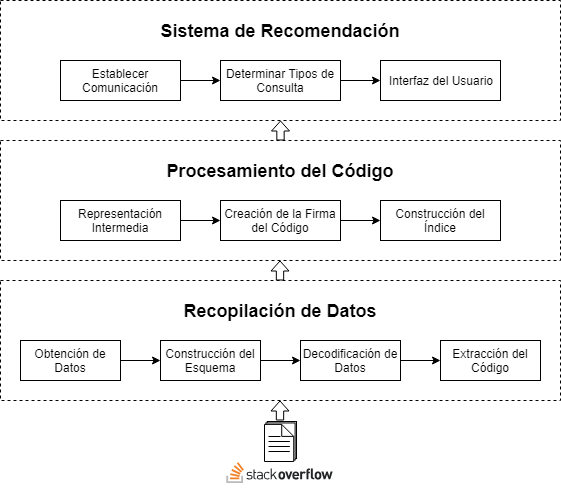
\includegraphics[width=30em]{img/metodo.png}
\caption{Esquema de Metodológico}
\label{fig:metodo}
\end{figure}

\section{Recopilación de Datos}
\label{sec:MedRecDat}

La información utilizada proviene de la base de
datos de \textit{Stack Overflow} del año $2014$,
es publicada en el formato \ac{XML} y
obtenida mediante el protocolo de transferencia \textit{BitTorrent}.
Además, es provista de forma libre bajo la licencia \textit{cc-by-sa 3.0},
que permite compartir y adaptar el contenido
si se atribuye el crédito a sus autores originales.

A continuación, se extraen los archivos de la base de datos y
la información es recopilada en \textit{PostgreSQL} para su posterior uso.

\subsection{Obtención de Datos}

Se obtienen y extraen los archivos \ac{XML} pertenecientes
a la base de datos de \textit{Stack Overflow},
los cuales se encuentran comprimidos en el formato \textit{7z},
utilizando la compresión \textit{bzip2}.
Una descripción detallada del contenido de los archivos 
se da en la Sección \ref{subsec:EstBasDat}.

\subsection{Construcción del Esquema}

Cada archivo \ac{XML} representa una tabla en la base de datos, 
donde los elementos bajo la etiqueta \textit{row} representan 
las filas y sus atributos representan las columnas.
Por este motivo, se utiliza \textit{PostgreSQL} para recopilar los datos,
ya que provee un conjunto de funciones para manipular texto en el formato \ac{XML}.

Estas funciones se emplean para desarrollar una serie de \textit{scripts}
en el lenguaje \ac{PL/pgSQL}, que permiten reproducir el esquema de
la base de datos de \textit{Stack Overflow}.

\subsection{Decodificación de Datos}

Los datos contienen entidades especiales en el formato \ac{XML}
que deben ser decodificadas para darle sentido a los tópicos.
Algunos de estas son: \lstinline{&amp;}, \lstinline{&lt;}, \lstinline{&gt;}.

Es de notar que la función \lstinline{xpath()} perteneciente a \textit{PostgreSQL},
es capaz de decodificar las entidades \ac{XML} al extraer los atributos de los elementos,
siempre que la versión de \textit{PostgreSQL} sea previa a la \textit{v9.2}~\cite{CAAY5AM3Cj}.

\subsection{Extracción del Código}

Un tópico %, ya sea éste una pregunta o una respuesta,
puede contener varios fragmentos de código dentro del cuerpo,
que se encuentra en formato \ac{HTML}.
Para extraer estos fragmentos,
se separa el texto contenido dentro de la etiqueta \lstinline{<code>}
y se almacena en una tabla independiente. 

Sin embargo, solo se consideran aquellos fragmentos de código que,
adicionalmente, se encuentran dentro de la etiqueta \lstinline{<pre>};
debido a que, dicha etiqueta es utilizada para mantener
el formato del texto, incluso si éste posee saltos de línea.

\section{Procesamiento del Código}
\label{sec:MedProcCod}

Los fragmentos de código extraídos son transformados en un conjunto de
\textit{n-grams}, lo que permite realizar comparaciones. Luego, 
a partir de esta representación se genera una firma,
que es mucho más compacta y eficiente.

\subsection{Representación Intermedia}
\label{subsec:MedRepInt}

Se emplea un \textit{lexer} para ignorar las modificaciones
de código de Tipo II, mencionados en la Sección \ref{subsec:plagio}.
De esta manera, se identifican los lexemas pertenecientes a los lenguaje c y c++ contenidos en 
el fragmento de código y se genera una secuencia de \textit{tokens}.

Luego, se utiliza la técnica de \textit{n-gram} para transformar la secuencia
de \textit{tokens}, en una representación intermedia que permite evaluar 
la similitud de dos fragmentos de código arbitrario mediante el coeficiente
de similitud de \textit{Jaccard}.

Finalmente, se utiliza una función de \textit{hash} para transformar los
\textit{n-grams} a enteros, permitiendo una representación más compacta
y una comparación más rápida.

\subsection{Creación de la Firma del Código}
\label{subsec:MedFirCod}

Se establece el tamaño de la firma y se calculan las funciones de \textit{hash}
asociadas. Luego, se genera la firma a partir del conjunto de \textit{n-grams}
utilizando el \textit{MinHash}, se almacena y se asocia al fragmento de código
correspondiente.% Dicha técnica, permite estimar el porcentaje de similitud,
%lo que evita operaciones costosas sobre conjuntos.

\subsection{Contrucción de un Índice}
\label{subsec:MedConInd}

Se establece la cantidad de bandas y su tamaño.
Luego, se separa cada firma en minifirmas,
usando la técnica de \ac{LSH}.
Entonces, se crea un índice invertido que almacena
las minifirmas en sus respectivas bandas
y las asocia al fragmento de código correspondiente.

Se puede abordar la creación de un índice invertido que
dependa de un entero si se utiliza una función de \textit{hash}
sobre los elementos de la minifirma.
Sin embargo, \textit{PostgreSQL} permite almacenar arreglos
de tamaño arbitrario y definir sus índices.

\section{Sistema de Recomendación}
\label{sec:MedConSisRec}

La elaboración del Sistema de Recomendación requiere establecer una estructura
de comunicación, determinar los tipos de consulta que se proveen y desarrollar
la interfaz gráfica.

\subsection{Establecer Comunicación}

Se calcula la firma del fragmento de código provisto por el usuario, 
siguiendo los pasos establecidos en las secciones:
Sección \ref{subsec:MedRepInt} y Sección \ref{subsec:MedFirCod}.
Luego, se construye la consulta y se envía al servidor de
bases de datos. El cual recibe la consulta y utiliza el
índice invertido desarrollado en la Sección \ref{subsec:MedConInd}
para retornar una lista de sugerencias.

\subsection{Determinar Tipos de Consulta}

Las consultas realizas por el \textit{Sistema de Recomendación} pueden
ser modificadas, permitiendo un mayor control sobre las 
sugerencias realizadas.

Las posibles modificaciones incluyen filtros que permitan
limitar las sugerencias, así como refinar la búsqueda
mediante el uso de distintas categorías.
Adicionalmente, se puede cambiar el orden por defecto,
ordenando los tópicos por reputación.

\subsection{Interfaz del Usuario}

El Sistema de Recomendación se provee con una interfaz
sencilla, que se compone de tres elementos.
Un botón de uso que permite capturar el fragmento de código
resaltado por el usuario, una ventana para
configurar las opciones de búsqueda y una 
ventana para mostrar las sugerencias.
\chapter{Desarrollo y Resultados}

En este capítulo se detallan los resultados obtenidos en la implementación y
ejecución del presente Proyecto de Grado. En primer lugar, en la Sección \ref{sec:DesRecDat},
se recopilan los datos en \textit{PostgreSQL}.
En segundo lugar, en la Sección \ref{sec:DesProCod}, se procesan los fragmentos 
de código, se crea la firma y se elabora el índice invertido. 
Posteriormente, en la Sección \ref{sec:DesConSisRec}, se crea el Sistema de Recomendación
y se muestran los resultados.

\section{Recopilación de Datos}
\label{sec:DesRecDat}

El peso aproximado de la base de datos de \textit{Stack Overflow} en formato \ac{XML}
es de $50GB$ para el año $2014$. 

\subsection{Obtención de Datos}

La base de datos contiene los siguientes archivos: 

\begin{itemize}
  \item \textit{Badges.xml}
  \item \textit{Comments.xml}
  \item \textit{PostHistory.xml} (\textbf{Ignorado})
  \item \textit{PostLinks.xml}
  \item \textit{Posts.xml} (\textbf{Necesario})
  \item \textit{Tags.xml} (\textbf{Necesario})
  \item \textit{Users.xml}
  \item \textit{Votes.xml}
\end{itemize}

\subsection{Construcción del Esquema}

El \textit{script} inicial recrea la estructura de las siguientes tablas:

\begin{itemize}
  \item \textit{Posts}
  \item \textit{PostCodes}
  \item \textit{PostTags}
  \item \textit{Tags}
\end{itemize}

Se puede encontrar el diagrama \textit{entidad-relación} en el Anexo \ref{ape:diag}.

Luego, los archivos \ac{XML} son procesados
mediante una serie de \textit{scripts} que 
tienen el nombre de la tabla correspondiente.
Estos \textit{scripts} se pueden encontrar en el Anexo \ref{ape:sql}
e incluyen la configuración sugerida para trabajar con
grandes volúmenes de datos.

El archivo \textit{Posts.xml} requiere la creación de la tabla \textit{PostTags},
para representar la relación \textit{many to many}, muchos a muchos,
que la tabla \textit{Post} guarda con respecto a la tabla \textit{Tags}.
Por otro lado, se considera la creación de la tabla \textit{PostCodes},
cuya relación es \textit{one to many}, uno a muchos,
para almacenar los fragmentos de código que son extraídos del tópico.

Estos \textit{scripts} se apoyan sobre la función \textit{xpath}
para extraer los atributos de los elementos y almacenarlos en los campos
correspondientes en su respectiva tabla.

El Fragmento de Código \ref{lst:example}, muestra un ejemplo de uso de la función
\lstinline{xpath()} para extraer el atributo de un elemento.

\begin{lstlisting}[caption={Función xpath.},label={lst:example}]
SELECT unnest(xpath('@Id', '<row Id="1" ... />')) as result;
 result
--------
 1
(1 fila)
\end{lstlisting}

Una vez almacenados los datos, se encuentra que existe un total de $21.736.593$ tópicos,
entre los cuales se consideran solo los que están relacionados con las etiquetas c y c++.
En consecuencia, la cantidad de tópicos utilizados a lo largo del Proyecto de Grado se limita a $1.420.664$.

En la Tabla \ref{tab:topicos} se muestra la cantidad de los tópicos relacionados con las distintas etiquetas.
\begin{table}[h]
\caption{Cantidad de tópicos por etiqueta.}
\label{tab:topicos}
\centering
\begin{tabular}{ccccc}
\hline
{Etiqueta} & {Preguntas} & {Respuestas} & \makecell{Respuestas\\Aceptadas} & {Total} \\
\hline
{todas} & $7.990.786$ & $13.684.117$ & $4.596.859$ & $21.736.593$ \\ 
{c/c++} & $442.450$ & $978.214$ & $284.297$ & $1.420.664$ \\ 
{c++} & $314.869$ & $684.362$ & $203.447$ & $999.231$ \\ 
{c} & $151.856$ & $362.244$ & $96.949$ & $514.100$ \\
\hline
\end{tabular}
\end{table}

Es importante destacar que, tan solo $284.297$ tópicos 
de este conjunto cuentan con una respuesta aceptada,
lo que representa un $29\%$ del total de las preguntas.
La búsqueda se limitaría significativamente si solo estas preguntas fuesen consideradas,
descartando tópicos relevantes para el usuario.

\subsection{Decodificación de Datos}
La decodificación de las entidades especiales 
se realizó empleando la clase \lstinline{StringEscapeUtils},
que contiene las funciones \lstinline{unescapeXml()} y \lstinline{unescapeHtml4()},
las cuales son usadas para decodificar texto en el formato 
\ac{XML} y \ac{HTML} respectivamente.
Esta clase pertenece a la librería mencionada en la Sección \ref{subsec:apache}.

La función \lstinline{unescapeXml()} se emplea para reemplazar
el contenido de los tópicos directamente en la base de datos. 
Mientras que la función \lstinline{unescapeHtml4()},
se utiliza para acceder al cuerpo del tópico.

\subsection{Extracción del Código}

Los fragmentos de código en los tópicos se encuentran bajo las etiquetas \ac{HTML} \lstinline{<pre>} o \lstinline{<code>},
de los cuales solo $773.320$ tópicos cumplen con el formato estándar.

Esto indica que al menos un $54.43\%$ de los tópicos relacionados con c y c++ contienen fragmentos de código,
siendo esta relación mayor en las preguntas ($71.02\%$) y menor en las respuestas ($46.93\%$).

\newpage
Un ejemplo del formato estándar se puede encontrar en el Fragmento de Código \ref{lst:top4},
extraído del tópico con \lstinline{Id = 4}.

\begin{lstlisting}[caption={Tópico Ejemplo.},label={lst:top4}]
...
<pre>
	<code>
		decimal trans = trackBar1.Value / 5000;
		this.Opacity = trans;
	</code>
</pre>
...
\end{lstlisting}

Existe un total de $1.377.716$ fragmentos de código, 
donde el $43.46\%$ se encuentra en las preguntas.
%Esto es un porcentaje importante, pues la cantidad de preguntas representa solo un $31.14\%$ de los tópicos.
%Lo que sugiere una mayor cantidad de fragmentos de código en las preguntas.


La Figura \ref{graf:distribucion} muestra las estadísticas 
descriptivas de los fragmentos de código por tópico,
se encuentra una media de 1 fragmento de código en las preguntas 
y 0 en las respuestas.
Por otra parte, la media es 1 para el total de los tópicos.

\begin{figure}[h]
\centering
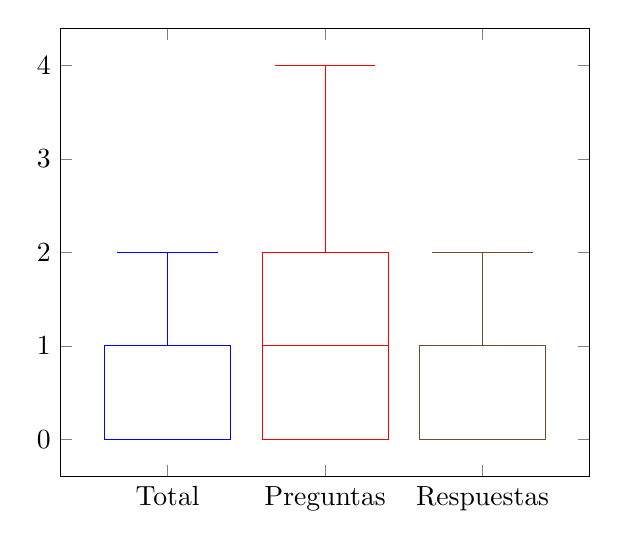
\begin{tikzpicture}
\begin{axis}[
boxplot/draw direction=y,
x=2cm,
xtick={1,2,3},
xticklabels={Total, Preguntas, Respuestas},
]
\addplot+ [boxplot prepared={
lower whisker=0,
lower quartile=0,
median=1,
upper quartile=1,
upper whisker=2}
%average=1},
] coordinates {};
\addplot+ [boxplot prepared={
lower whisker=0,
lower quartile=0,
median=1,
upper quartile=2,
upper whisker=4}
%average=1},
] coordinates {};
\addplot+ [boxplot prepared={
lower whisker=0,
lower quartile=0,
median=0,
upper quartile=1,
upper whisker=2}
%average=0},
] coordinates {};
% \addplot+ [boxplot prepared={
% lower whisker=1,
% lower quartile=1,
% median=1,
% upper quartile=2,
% upper whisker=31},
% ] coordinates {};
% \addplot+ [boxplot prepared={
% lower whisker=1,
% lower quartile=1,
% median=1,
% upper quartile=2,
% upper whisker=42},
% ] coordinates {};
\end{axis}
\end{tikzpicture}
\caption{Estadísticas descriptivas de los fragmentos de código.}
\label{graf:distribucion}
\end{figure}


Se aprecia que la cantidad de líneas en los fragmentos de código pertenecientes a las preguntas suele ser mayor,
esto se evidencia al analizar la Figura \ref{graf:lineas}.
Donde se muestra una media de 8 líneas de código en las preguntas y 4 en las respuestas,
mientras que la media general es 5.

\begin{figure}[h]
\centering
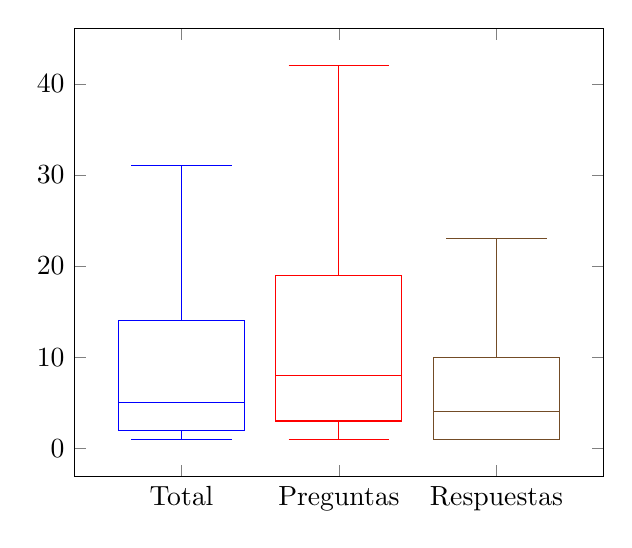
\begin{tikzpicture}
\begin{axis}[
boxplot/draw direction=y,
x=2cm,
xtick={1,2,3},
xticklabels={Total, Preguntas, Respuestas},
]
\addplot+ [boxplot prepared={
lower whisker=1,
lower quartile=2,
median=5,
upper quartile=14,
upper whisker=31},
%upper whisker=1266},
] coordinates {};
\addplot+ [boxplot prepared={
lower whisker=1,
lower quartile=3,
median=8,
upper quartile=19,
upper whisker=42},
%upper whisker=1266},
] coordinates {};
\addplot+ [boxplot prepared={
lower whisker=1,
lower quartile=1,
median=4,
upper quartile=10,
upper whisker=23},
%upper whisker=1236},
] coordinates {};
\end{axis}
\end{tikzpicture}
\caption{Estadísticas descriptivas de las líneas de código.}
\label{graf:lineas}
\end{figure}


\section{Procesamiento del Código}
\label{sec:DesProCod}

Como han indicado \cite{monperrus:hal-00987395},
el motor de búsqueda de \textit{Stack Overflow} no es adecuado para realizar consultas utilizando fragmentos de código.
Debido a esto, se aplicó la técnica de \ac{LSH} para crear un índice especializado.

\subsection{Representación Intermedia del Código}
\label{subsec:DesIntCod}

Antes de transformar el código, se debe tener algunas consideraciones en cuenta:

\begin{itemize}
  \item Existen caracteres reservados en el formato \ac{HTML}, que deben ser decodificados.
  Algunos de estos son: \lstinline{&amp;}, \lstinline{&nbsp;}, \lstinline{&#64;}.

  \item Se deben eliminar todas las directivas de preprocesamiento, no son significativas.
  Como por ejemplo: \lstinline{#include <cstring>}.
  
  \item No es necesario preocuparse por los comentarios, el \textit{lexer} se encargará de ellos.
  Tal es el caso de: \lstinline{// This is a valid comment}.
\end{itemize}

El \textit{lexer} se encarga de identificar los lexemas como enteros en el rango de $1$ a $144$.
Se encontró que la mitad de ellos no se usan, ya que son asignados por el \textit{paser}
o han sido marcados como obsoletos. Una lista detallada de estos lexemas
puede consultarse en el Anexo \ref{ape:tok}.

\newpage
El \textit{lexer} identifica los lexemas en el Fragmento de Código \ref{lst:fc4} 
y los separa en una serie de \textit{tokens} de la siguiente manera:

\begin{verbatim}
 identifier, identifier, assign, identifier, dot, identifier, div, integer,
        semi, identifier, dot, identifier, assign, identifier, semi
\end{verbatim}

\begin{lstlisting}[caption={Fragmento de código en c++},label={lst:fc4}]
decimal trans = trackBar1.Value / 5000;
this.Opacity = trans;
\end{lstlisting}
Estos \textit{tokens} son representados por enteros, tal que:

\begin{verbatim}
             1, 1, 38, 1, 50, 1, 52, 2, 5, 1, 50, 1, 38, 1, 5
\end{verbatim}

Luego, se utiliza la técnica de \textit{n-grams} sobre el Fragmento de Código
\ref{lst:fc4} con $n = 4$, ya que ha mostrado los mejores resultados~\cite{Burrows:2007:EPD:1228662.1228664}.
Obteniéndose la siguiente secuencia:

\begin{verbatim}
(1,1,38,1), (1,38,1,50), (38,1,50,1), (1,50,1,52), (50,1,52,2), (1,52,2,5),
 (52,2,5,1), (2,5,1,50), (5,1,50,1), (1,50,1,38), (50,1,38,1), (1,38,1,5)
\end{verbatim}

Posteriormente, se suele usar una función de \textit{hash}
para transformar la secuencia de \textit{n-grams} en una secuencia de enteros.
Sin embargo, dada la naturaleza de estos \textit{n-grams}, 
se pueden almacenar sus valores en enteros sin colisiones;
dado a que existen $429.981.695$ combinaciones
en el conjunto de los \textit{4-grams}, al que se denomina $G$.

Luego, como $G$ es finito, es un conjunto numerable; 
por lo tanto, existe una función $f$ inyectiva al conjunto de los naturales, tal que:
\begin{equation*}
f : G \rightarrow\mathbb{N}
\end{equation*}
Tal función se escribe:
\begin{equation*}
f(G) = (G_3-1) * 144^3 + (G_2-1) * 144^2 + (G_1-1) * 144^1 + (G_0-1)*144^0
\end{equation*}

%Por ejemplo, al representar el \textit{} $(1,1,38,1)$ como un entero, se tiene:

%\begin{equation*}
%5328 = (1-1) * 144^3 + (1-1) * 144^2 + (38-1) * 144^1 + (1-1)*144^0
%\end{equation*}

Luego, para el Fragmento de Código \ref{lst:fc4} se obtiene la siguiente representación:

\begin{verbatim}

  5328, 767281, 110488464, 1016115, 146320561, 1057684, 152306496, 3068977,
               11950992, 1016101, 146318544, 767236, 110482127
\end{verbatim}

\subsection{Creación de la Firma del Código}
\label{subsec:DesFirCod}

Se escogen $100$ funciones de \textit{hash} para la elaboración
de la firma mediante la técnica de \textit{MinHash},
tal que el error esperado es a lo sumo un $10\%$.
Continuando con el Fragmento de Código \ref{lst:fc4} que usamos como ejemplo,
se procede a generar la firma.

Se escogen las siguientes funciones de \textit{hash}:
\begin{gather*}
f_1(x) = (x * 133 + 2.163) \bmod 429.981.701 \\
f_2(x) = (x * 140.002 + 1.234) \bmod 429.981.701\\
\vdots \\
f_{100}(x) = (x * 91.231.268 + 300.122.522) \bmod 429.981.695
\end{gather*}
	
%A su vez, se escogen los coeficientes $a=140.002$ y $b=1.234$, se tiene:

%\begin{equation*}
%f_2(x) = (x * 140.002 + 1.234) \bmod 429.981.701
%\end{equation*}

%\begin{equation*}
%\vdots
%\end{equation*}

%Finalmente, se escogen los coeficientes $a = 91.231.268$ y $b = 300.122.522$, se tiene:

%\begin{equation*}
%f_{100}(x) = (x * 91.231.268 + 300.122.522) \bmod 429.981.695
%\end{equation*}

Al aplicar estas funciones de \textit{hash} sobre el Fragmento de Código \ref{lst:fc4}, se obtienen los valores:
\begin{gather*}
f_1(x) \rightarrow \{604227, 86704916, 15729266, 114823158, 194920918, 119520455,\\
							  11368171, 346796564, 60519156, 114821576, 194692997, 86699831, 15013185\}\\
f_2(x) \rightarrow \{315950189, 355432247, 14244687, 364172134, 412965015, 164171458,\\
							  421501636, 111199889, 103984627, 362212106, 130580981, 349132157, 416997116\}\\
\vdots\\
f_{100}(x) \rightarrow \{181460756, 87946214, 32252656, 301023389, 176237545, 260167737,\\
									 323195011, 209406491, 271127092, 17027248, 139482376, 127203813, 324373383\}
\end{gather*}

Luego, la firma para el Fragmento de Código \ref{lst:fc4} estaría conformada por los mínimos:
\begin{gather*}
firma(C_1) = (604227, 14244687, \dots, 17027248)
\end{gather*}

En el proceso se descartó $48.028$ fragmentos nulos, persistiendo $1.329.688$.
De los cuales, $581.798$ se asocian con preguntas y $747.890$ se asocian con respuestas.

\subsection{Construcción de un Índice}
\label{subsec:DesConInd}

La configuración inmediata para el \ac{LSH} consiste en dividir las
firmas cuyo tamaño es $100$, en $20$ bandas con $5$ filas cada una.
Esto da como resultado un umbral de similitud aproximado del $54.93\%$,
que los fragmentos de código tienen que superar para convertirse en pares candidatos.

La creación del índice produjo un total de $26.593.760$
entradas en la base de datos, las cuales se distribuyen entre las bandas.
Cada banda está conformada por $1.329.688$ minifirmas,
que se emplean como claves y se asocian a un fragmento de código.

\subsubsection{Evaluación del Índice Invertido}

Para comprobar la funcionalidad del índice,
se escogió un total de $1.000$ fragmentos de código escogidos al azar de forma uniforme,
los cuales fueron extraídos directamente de la base de datos y
se identifican como conjunto $1$. Este conjunto se puede consultar en el Anexo \ref{ape:conj}.


\begin{itemize}
  \item $1.000/1.000$ tópicos encontrados.
  \item $730/1.000$ tópicos encontrados en el primer lugar.
  \item $122/1.000$ tópicos encontrados entre los diez primeros.
  \item $148/1.000$ tópicos encontrados en alguna otra posición.
\end{itemize}

Las pruebas realizadas sobre el conjunto $1$,
se usan para evaluar la efectividad al seleccionar un tópico.
Los resultados muestran que cualquier fragmento de código indexado correctamente,
es considerado par candidato y por consiguiente encontrado.

Se utilizan las firmas para evaluar la similitud entre los fragmentos de código,
todos los fragmentos se evaluaron con una similitud del $100\%$.
Si se usa el coeficiente de similitud de \textit{Jaccard} para comparar los fragmentos los resultados apenas varían,
modificando un solo tópico; el tópico modificado pasaría del 2\textsuperscript{do} al 1\textsuperscript{er} lugar,
debido a que un tópico similar que se encontraba en la primera posición dejo de tener una similitud del 100\%.

Las pruebas realizadas arrojaron datos estimados del tiempo de búsqueda,
cuyo promedio es $194$ milisegundos. Gran parte del tiempo es invertido
en la consulta realizada, cuyo promedio es $185$ milisegundos.
Son encontrados $500$ pares candidatos en promedio y
el tiempo empleado para evaluar cada firma es de $0.28$ milisegundos aproximadamente.



%La certeza de cuán parecidos son los fragmentos de código, es obtenida a través del \textit{MinHash}.
%Lo que implica que dos fragmentos cualesquiera, cuya estructura sea idéntica, 
%tendrán la misma ponderación al ser comparados con un tercer fragmento.
%Por lo tanto, el orden en el que aparecen los fragmentos de código estructuralmente iguales, es arbitrario.

Para evaluar la capacidad de búsqueda de fragmentos de código arbitrario,
se utilizó un conjunto de  $195$ fragmentos extraidos de una fuente externa,
al que se identifica como conjunto $2$. El origen de este conjunto se especifica en el Anexo \ref{ape:conj}.

Estos fragmentos de código no guardan relación con la base de datos de \textit{Stack Overflow} y
se utilizan para determinar la viabilidad al realizar consultas con fragmentos arbitrarios.

Se estableció una clasificación basada en la similitud estructural de los fragmentos de código.
Aquellos fragmentos de código cuya similitud es igual o superior
al $95\%$, se clasifican en el rango $1$, si es igual o superior
al $85\%$, se clasifican en el rango $2$, si es igual o superior
al $70\%$, se clasifican en el rango $3$ y si es igual o superior
al $50\%$, se clasifican en el rango $4$.
 
Los resultados encontrados al aplicar esta clasificación al conjunto de
fragmentos de código arbitrario, se encuentran en la Tabla \ref{tab:clasificacion}.

\begin{table}[h]
\caption{Clasificación de Fragmentos de Código.}
\label{tab:clasificacion}
\centering
\begin{tabular}{ccccc}
\hline
{Rango 1} & {Rango 2} & {Rango 3} & {Rango 4} & {Sin rango} \\
\hline
$12$ & $8$ & $20$ & $55$ & $100$ \\
\hline
\end{tabular}
\end{table}

A continuación, se detallan las características encontradas en cada rango:

\begin{description}
  \item [Rango 1] Son fragmentos de código considerados estructuralmente iguales.
  Pueden haber variaciones en la cardinalidad de los \textit{n-gram}.
  Esto se traduce, en secuencias de tamaño $n$ repetidas.
  \item [Rango 2] Son fragmentos de código con inserciones de una o más constantes,
  variables u operadores que modifican pocos \textit{n-gram}, típicamente de $3$ a $7$.
  \item [Rango 3] Son fragmentos de código que poseen cambios estructurales básicos,
  dependiendo de la longitud del código se muestran en mayor o menor grado.
  \item [Rango 4] Son fragmentos de código que poseen cambios estructurales importantes,
  en general difieren mucho del fragmento de código considerado.
  \item [Sin rango] Son fragmentos de código con muy poca o ninguna similitud.
\end{description}

A efectos de la evaluación de los fragmentos de código se define la especificidad
de un fragmento de código, como la cantidad de líneas de código que éste posee.
Sin definir una cantidad precisa, se dirá que a mayor especificidad, mayor cantidad de líneas de código.

La Figura \ref{graf:lineas2} muestran un crecimiento lineal en el conjunto $2$,
que involucra a los fragmentos código del rango $2$ en adelante.
Dicho comportamiento sugiere que la especificidad de los fragmentos de código,
disminuye la probabilidad de encontrar otros fragmentos estructuralmente iguales o similares.

\begin{figure}[h]
\centering
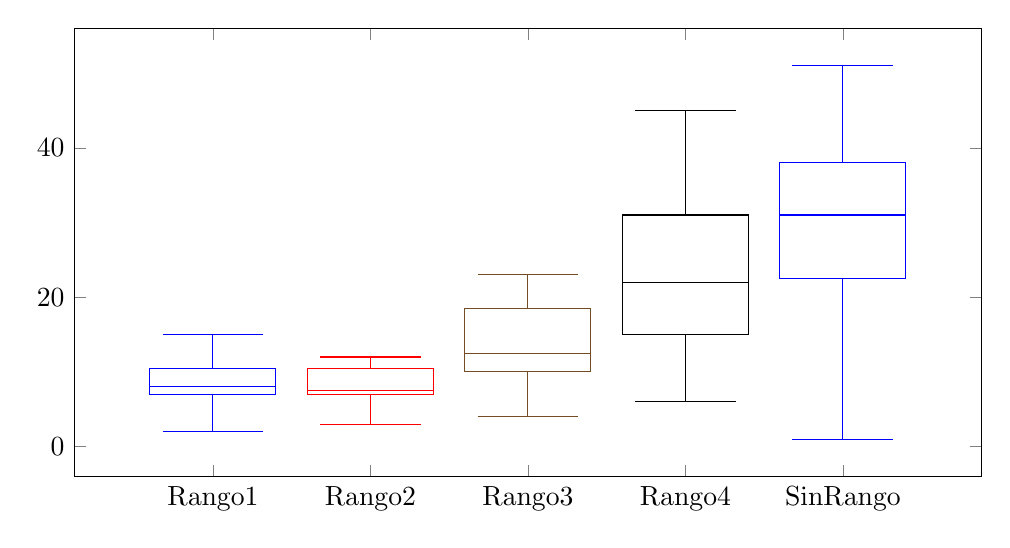
\begin{tikzpicture}
\begin{axis}[
boxplot/draw direction=y,
x=2cm,
xtick={1,2,3,4,5},
xticklabels={Rango1, Rango2, Rango3, Rango4, SinRango},
]
\addplot+ [boxplot prepared={
lower whisker=2,
lower quartile=7,
median=8,
upper quartile=10.5,
upper whisker=15},
] coordinates {};
\addplot+ [boxplot prepared={
lower whisker=3,
lower quartile=7,
median=7.5,
upper quartile=10.5,
upper whisker=12},
] coordinates {};
\addplot+ [boxplot prepared={
lower whisker=4,
lower quartile=10,
median=12.5,
upper quartile=18.5,
upper whisker=23},
%upper whisker=34},
] coordinates {};
\addplot+ [boxplot prepared={
lower whisker=6,
lower quartile=15,
median=22,
upper quartile=31,
upper whisker=45},
] coordinates {};
\addplot+ [boxplot prepared={
lower whisker=1,
lower quartile=22.5,
median=31,
upper quartile=38,
upper whisker=51},
] coordinates {};
\end{axis}
\end{tikzpicture}
\caption{Estadísticas descriptivas de las líneas de código.}
\label{graf:lineas2}
\end{figure}

Se hace notar que los fragmentos de código que se encuentran en el rango $2$ y posterior,
no tienen una estructura equivalente dentro de la base de datos.
Esto se desprende de las pruebas realizadas sobre el conjunto $1$,
donde todos los fragmentos de código se corresponden al rango $1$.

Sin embargo, existen muchos más fragmentos de código en el rango $1$ que en el rango $2$.
Lo que sugiere que una media de 8 líneas de código es lo apropiado para 
encontrar estructuras equivalentes dentro de la base de datos.

Luego, al evaluar los fragmentos de código en el rango $8\pm1$, se encuentran solo 16 fragmentos
y como se evidencia en la Tabla \ref{tab:clasificacion2}, la probabilidad de que un fragmento
con 8 líneas de código se encuentre en el rango $1$ es de $37.5\%$, en el rango $2$ es
de $25.0\%$, en el rango $3$ es de $18.75\%$, en el rango $4$ es de $6.25\%$ y no tenga rango
es de $12.5\%$ para el conjunto $2$.

\begin{table}[h]
\caption{Clasificación de Fragmentos de Código en el rango $8\pm1$.}
\label{tab:clasificacion2}
\centering
\begin{tabular}{ccccc}
\hline
{Rango 1} & {Rango 2} & {Rango 3} & {Rango 4} & {Sin rango} \\
\hline
$6$ & $4$ & $3$ & $1$ & $2$ \\
\hline
\end{tabular}
\end{table}

\section{Sistema de Recomendación}
\label{sec:DesConSisRec}

El Sistema de Recomendación propuesto se implementa como
un \textit{plug-in} de \textit{Eclipse}, que se comunica mediante
un esquema \textit{cliente-servidor} y realiza consultas directamente
al servidor de base de datos \textit{PostgreSQL}.
Este proceso se muestra en la Figura \ref{fig:diag1}.

\begin{figure}[h]
\centering
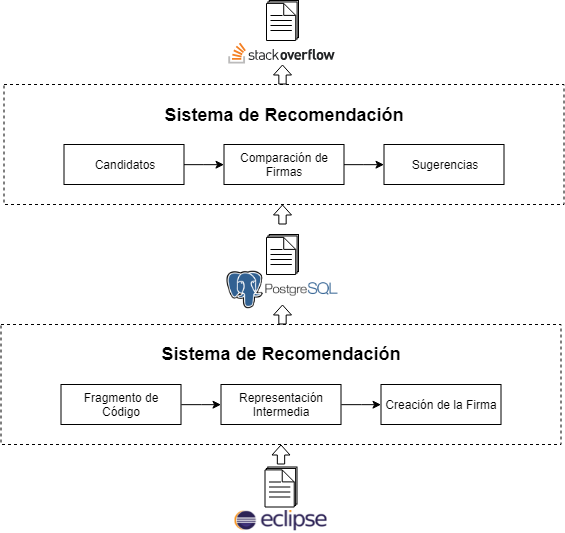
\includegraphics[width=30em]{img/comunicacion.png}
\caption{Estructura de Comunicación}
\label{fig:diag1}
\end{figure}

\subsection{Establecer Comunicación}

El Sistema de Recomendación 
captura el fragmento de código provisto por el usuario y sigue los pasos 
establecidos en las secciones: Sección \ref{subsec:DesIntCod} y Sección \ref{subsec:DesFirCod}.
Entonces, el fragmento de código es transformado en una serie de \textit{tokens}
mediante el \textit{lexer}, los cuales son agrupados para formar \textit{4-grams}
y se calcula la firma a partir de ellos.
%Entonces, la clase \textit{Tokenizer} recibe el fragmento de código 
%y lo pasa al \textit{lexer}, retornando un \textit{iterador}.
%El \textit{iterador} es recorrido obteniendo una serie de \textit{tokens},
%los cuales son agrupados para formar \textit{4-grams} y se calcula el valor de
%cada uno mediante la clase \textit{Ngram}, produciendo un conjunto de enteros;
%ésta es la Representación Intermedia del código.
%La clase \textit{MinHash} recibe el conjunto de enteros y
%genera la firma con los mínimos obtenidos al multiplicar las funciones de \textit{hash}.
Luego, el Sistema de Recomendación construye la consulta con la firma obtenida 
y la envía al servidor de bases de datos.

Posteriormente, el servidor de bases de datos recibe la consulta y separa
la firma en minifirmas. Se usa el índice invertido, desarrollado en la
Sección \ref{subsec:DesConInd}, para buscar los pares candidatos
mediante las minifirmas. Luego, se forma una lista con los pares candidatos
encontrados que incluye sus firmas y el servidor la envía al cliente.

Finalmente, el cliente recibe la lista y compara las firmas. De esta manera,
construye las sugerencias en base a la similitud de los pares candidatos,
mostrando solo aquellos que cumplen con los parámetros establecidos.


\subsection{Determinar Tipos de Consulta}

Las sugerencias realizas se pueden limitar a un subconjunto especifico 
de tópicos, entre los cuales se encuentran las preguntas y las respuestas.
A su vez, la consulta de preguntas puede ser restringida a aquellas
que tengan una respuesta aceptada, mientras que la consulta de respuestas
puede ser restringida a aquellas que han sido aceptadas.

En la Sección \ref{subsec:DesConInd}, se estableció una clasificación
en base a la similitud de los fragmentos de código, que describe las
características de cada rango. Esta clasificación es empleada
para filtrar los resultados mostrados en las sugerencias.

El orden por defecto en el que se muestran los tópicos está dado
por la similitud de los fragmentos de código que éstos contienen.
Sin embargo, es posible ordenar la lista de sugerencias en base
a la reputación de los tópicos.

\subsection{Interfaz del Usuario}

El Sistema de Recomendación se provee con una interfaz
sencilla, compuesta de tres elementos describen a continuación.
La Figura \ref{fig:srse} muestra dicha interfaz.

El botón de consulta dispara un evento que captura
el fragmento de código resaltado por el usuario,
inmediatamente se muestra la ventana de consulta.

La ventana de consulta permite especificar los 
parámetros de búsqueda, entre los que se encuentran:
los filtros a aplicar sobre los tópicos, 
las categorías en las que se hallan
y el orden en el que se muestran.
%Esta ventana contiene un botón para enviar
%y otro para cancelar.

La ventana de sugerencias muestra la lista de
los tópicos de \textit{Stack Overflow} propuestos.
Se compone del tipo del tópico, el título,
la reputación y el porcentaje de similitud.

\begin{figure}[h]
\centering
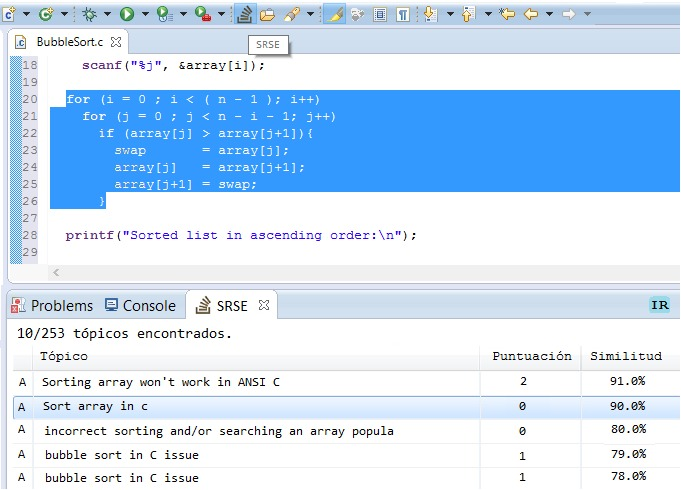
\includegraphics[width=30em]{img/srse.jpg}
\caption{Interfaz del Usuario}
\label{fig:srse}
\end{figure}

% \subsection{Ejemplo de uso}


% Si tomamos una implementación típica, como lo es \textit{bubble sort},
% que se muestra en la Figura \ref{lst:bubble} obtendremos como sugerencias,
% los resultados que se muestran en la Figura \ref{lst:rbubble}.

% \begin{lstlisting}[caption={Bubble Sort.},label={lst:bubble}]
% for (c = 0 ; c < ( n - 1 ); c++)
	% for (d = 0 ; d < n - c - 1; d++) {
		% if (array[d] > array[d+1]) {
			% swap       = array[d];
			% array[d]   = array[d+1];
			% array[d+1] = swap;
		% }
% \end{lstlisting}

% \begin{lstlisting}[caption={Resultados Bubble Sort.},label={lst:rbubble}]
% 1) A:Sorting array won't work in ANSI C (2) 91.0%
% 2) A:Sort array in c (0) 90.0%
% 3) A:incorrect sorting and/or searching an array popula (0) 80.0%
% 4) A:bubble sort in C issue (0) 79.0%
% 5) A:bubble sort in C issue (1) 78.0%
% 6) A:bubble sort in C issue (1) 77.0%
% 7) A:Sorting gives inconsistent results, due to loop bo (0) 75.0%
% 8) A:Recursive Bubble Sort in C (1) 73.0%
% 9) Q:Time Computational complexity? (-3) 73.0%
% 10) Q:Undefined behaviour while swapping/exchanging poin (0) 71.0%
% \end{lstlisting}

% Si en cambio, seleccionamos la implementación completa de \textit{bubble sort}
% como se muestra en la Figura \ref{lst:bubblec} obtendremos como sugerencias,
% los resultados que se muestran en la Figura \ref{lst:rbubblec}.

% \begin{lstlisting}[caption={Bubble Sort Completo.},label={lst:bubblec}]
% void main() {
	% int array[100];
	% int i, j, n, swap;
	% scanf("%d", &n); // Enter number of elements
	% for (i = 0; i < n; i++) // Enter integers
		% scanf("%d", &array[i]);
	% for (i = 0; i < n - 1; i++)
		% for (j = 0 ; j < n - i - 1; j++) {
			% if (array[j] > array[j+1]) {
				% swap       = array[j];
				% array[j]   = array[j+1];
				% array[j+1] = swap;
			% }
	% for (i = 0; i < n; i++) // Print ordered list
		% printf("%d\n", array[i]);
% }
% \end{lstlisting}

% \begin{lstlisting}[caption={Resultados Bubble Sort completo.},label={lst:rbubblec}]
% 45 resultados encontrados.
% 1) Q:I made this program for sorting of n numbers in C, (0) 71.0%
% 2) Q:warning: comparison between pointer and integer an (2) 68.0%
% 3) Q:The program wont work for n>9... It works fine whe (0) 67.0%
% 4) Q:Unable to run this code still it shows no errors? (0) 67.0%
% 5) Q:Can't find most frequent word (3) 65.0%
% 6) Q:What's wrong with my for-loop? (1) 65.0%
% 7) Q:Calculating a Percentile (1) 61.0%
% 8) A:Bubble Sort in C (2) 61.0%
% 9) Q:Merge 2 arrays and omit all repeating elements (0) 61.0%
% 10) Q:adding an extra number to be sorted (0) 61.0%
% \end{lstlisting}

\subsection{Evaluación del Sistema de Recomendación}

Se seleccionó un conjunto de 10 elementos, llamado conjunto 3,
que contiene algoritmos de variado propósito,
la prueba cumple con las siguientes condiciones:

\begin{itemize}
	\item Algoritmos completos seleccionados al azar.
	\item Se verifican solo los 10 primeros resultados.
	\item Se verifican solo si su similitud es mayor al 50.\%.
	\item El resultado de los tópicos se clasifica en 3 áreas, encontrado, relacionado, no encontrado;
	para alguno de los tópicos en ese orden.
\end{itemize}

\begin{lstlisting}[caption={Alexander Bogomolny.},label={lst:alex}]
3 resultados encontrados.
1) A:All possible combinations of n items selected rand (0) 83.0%
2) A:Creating every possible value of a fixed size arra (0) 83.0%
3) A:Generating all size k subsets of {0, 1, 2, ... n-1 (1) 53.0%
\end{lstlisting}

\newpage
\begin{lstlisting}[caption={Bin Packing.},label={lst:binpack}]
6 resultados encontrados.
1) Q:Read and Display matrix (0) 55.0%
2) Q:"for" loop inside a switch case doesn't work (0) 53.0%
3) A:Prime number generation algorithm (-2) 52.0%
4) Q:returning a floating point value from a function (1) 51.0%
5) Q:nth root of a number (6) 50.0%
6) Q:Segmentation Fault Error; Absolute Value Table (0) 50.0%
\end{lstlisting}

\begin{lstlisting}[caption={Binary Search Tree.},label={lst:binsearch}]
47 resultados encontrados.
1) Q:errors in delete function of binary search tree (-1) 64.0%
2) Q:AddNew Function using Linked List In C (0) 60.0%
3) Q:Getting error in deleting a node in a linked list  (0) 59.0%
4) Q:Nested Functions are disabled, use -fnested-functi (-2) 57.9%
5) Q:segmentation fault while implementing the binary t (-1) 56.9%
6) Q:Printing Reversed linked list iteratively (3) 56.0%
7) Q:Showing Error Segmentation fault (-7) 56.0%
8) Q:C Program to copy one binary search tree to anothe (1) 56.0%
9) Q:Write a function in c with which we can add more t (-1) 56.0%
10) Q:Binary search tree Segfault (-1) 56.0%
\end{lstlisting}

\begin{lstlisting}[caption={Fisher Yates.},label={lst:yates}]
2 resultados encontrados.
1) A:Is this C implementation of Fisher-Yates shuffle c (22) 63.0%
2) Q:Shuffle a struct (2) 63.0%
\end{lstlisting}

\begin{lstlisting}[caption={Knapsack Problem.},label={lst:knapsack}]
1 resultados encontrados.
1) Q:Knapsack 1/0 Implementation needs explanation (0) 94.0%
\end{lstlisting}

\newpage
\begin{lstlisting}[caption={Selection Sort.},label={lst:selec}]
6 resultados encontrados.
1) A:array in descending order doesn't work in C (4) 68.0%
2) A:C Sorting an array by integer (1) 61.0%
3) Q:Passing an array as an argument to a function poin (0) 54.0%
4) Q:trouble reading a 2D array of characters in C? (0) 51.0%
5) Q:Factorial -C (Linux) (1) 50.0%
6) Q:How to check if the elements in the main diagonal  (0) 50.0%
\end{lstlisting}

\begin{lstlisting}[caption={The Sieve of Eratosthenes.},label={lst:sieve}]
2 resultados encontrados.
1) Q:The Sieve of Eratosthenes code in C (0) 78.0%
2) Q:Dynamic memory array crash the executable (1) 53.0%
\end{lstlisting}

Los resultados obtenidos se muestran en la Tabla \ref{tab:res3},
junto con el número de líneas,
la cantidad de candidatos y
el mayor porcentaje obtenido.

\begin{table}[h]
\caption{Resultados conjunto C.}
\label{tab:res3}
\centering
\begin{tabular}{ccccc}
\hline
{Algoritmo} & {Resultado} & {Líneas} & {Candidatos} & {Porcentaje} \\
\hline
Alexander Bogomolny & $Encontrado$ & $36$ & $3$ & $83\%$ \\
Bin Packing & $No encontrado$ & $30$ & $6$ & $55\%$ \\
Binary Search Tree & $Encontrado$ & $163$ & $47$ & $64\%$ \\
Fibonacci Search & $No Encontrado$ & $48$ & $0$ & $0\%$ \\
Fisher Yates & $Encontrado$ & $33$ & $2$ & $63\%$ \\
Hash Table & $No Encontrado$ & $184$ & $0$ & $0\%$ \\
0-1 Knapsack Problem & $Encontrado$ & $78$ & $1$ & $94\%$ \\
Naor Reigngold & $No Encontrado$ & $17$ & $0$ & $0\%$ \\
Selection Sort & $Encontrado$ & $41$ & $6$ & $68\%$ \\
Sieve Eratosthenes & $Encontrado$ & $22$ & $2$ & $78\%$ \\
\hline
\end{tabular}
\end{table}

Se confirman varios aspectos resaltados en la Sección \ref{subsec:DesConInd}.
En primer lugar, si existen estructuras equivalentes o idénticas, 
el Sistema de Recomendación las encuentra.
Lo que se puede apreciar en el resultado obtenido por el código \textit{0-1 Knapsack Problem},
cuya especificidad es alta, tiene un gran porcentaje de similitud y es el único encontrado.
En segundo lugar, la especificidad disminuye la probabilidad de encontrar fragmentos de código similares.
Lo que se desprende de los resultados obtenidos por el código \textit{Tabla de Hash} y el código \textit{Binary Search Tree},
implementaciones que suelen ser muy comunes y sin embargo, solo fue posible encontrar uno de ellos.

En la Tabla \ref{tab:resss3} se muestran los resultados finales obtenidos,
se aprecia una efectividad del $60.0\%$ al evaluar códigos completos.
Sin embargo, estos códigos son muy comunes y se espera que el porcentaje 
baje ante una implementación propia.

\begin{table}[H]
\caption{Resultados Conjunto 3}
\label{tab:resss3}
\centering
\begin{tabular}{ccc}
\hline
{Resultado} & {Cantidad} & {Porcentaje} \\
\hline
$Encontrado$ & $6$ & $60.0\%$ \\
$No Encontrado$ & $4$ & $40.0\%$ \\
$Relacionado$ & $0$ & $0.0\%$ \\
\hline
\end{tabular}
\end{table}


\chapter*{Conclusiones y Recomendaciones}

En el presente Proyecto de Grado se propuso la creación de un Sistema de Recomendación,
que se apoye sobre algoritmos de minería de datos para proveer sugerencias en tiempo real.
Estas sugerencias se realizan en base al fragmento de código provisto por el usuario en lenguaje c y c++,
el cual se hace coincidir con fragmentos de código que se encuentran en los tópicos de \textit{Stack Overflow}.

El sistema implementado demostró funcionar correctamente al sugerir tópicos,
cuyos fragmentos de código, son estructuralmente iguales o similares al proporcionado por el usuario.

Se encontraron los siguientes resultados parciales en la ejecución del presente proyecto:

\begin{itemize}
  \item El índice desarrollado en este proyecto es eficaz al obtener fragmentos de código que se encuentren previamente en la base de datos.
  \item Los fragmentos de código con baja especificidad tienen una mayor incidencia en los tópicos,
  lo que permite encontrar otros fragmentos iguales o similares estructuralmente con mayor probabilidad.
  Se encontró que $8$ líneas de código en promedio ofrece los mejores resultados.
\end{itemize}

El enfoque innovador utilizado en este proyecto,
se basa en la similitud sintáctica de los fragmentos de código para realizar sugerencias;
siendo en esencia, una comparación estructural pura.

Sin embargo, se subraya el hecho de que cualquier par de fragmentos de código,
estructuralmente iguales, pueden no poseer el mismo comportamiento.
Esto ocurre generalmente cuando la especificidad de los fragmentos es baja.

La lista de tópicos desplegada por la herramienta puede ser configurada,
restringiendo el espacio de búsqueda y alineando los resultados a los intereses del usuario.

El usuario puede dar preferencia a la búsqueda de preguntas o respuestas.
Además, es posible limitar la búsqueda a las preguntas con respuesta aceptada o a las respuestas aceptadas.
Así como, ordenar los resultados de acuerdo a la reputación del tópico.

De los resultados obtenidos se derivan los siguientes aspectos para su posterior estudio:

\begin{itemize}
  \item Expandir el preprocesamiento de los datos para incluir fragmentos de código que no se encuentren en el formato estándar.
  \item Ampliar el análisis sintáctico incluyendo el uso de un \textit{parser}, con la finalidad de incrementar la precisión.
  \item Implementar una función de \textit{hash} en el índice, con la finalidad de acelerar el proceso de búsqueda.
  \item Desarrollar una clasificación automática de los resultados mediante filtros especializados que incluyan información del contexto.
  \item Investigar algoritmos que permitan evaluar la contención de conjuntos, de forma similar a como se evalúa la igualdad de conjuntos mediante el \textit{MinHash}.
\end{itemize}
\bibliography{referencias}

\appendix
\chapter{Diagrama Base de Datos}
\label{ape:diag}

\begin{figure}[h]
\centering
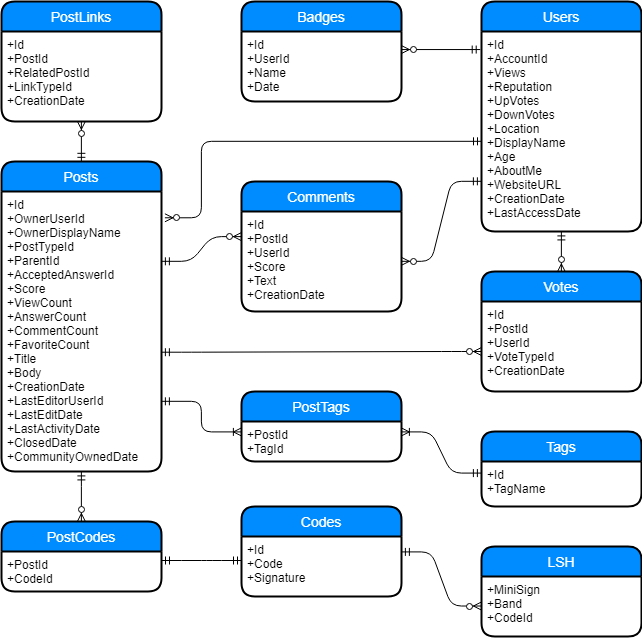
\includegraphics[width=36em]{img/er.png}
\caption{Diagrama Entidad-Relación}
\label{fig:er}
\end{figure}

%Se puede encontrar el esquema general de la base de datos en el siguiente enlace:

%\url{https://meta.stackexchange.com/questions/2677/database-schema-documentation-for-the-public-data-dump-and-sede}

\begin{table}[h]
\caption{Campos de la Tabla Badges.}
\centering
\begin{tabular}{ccc}
\hline
Nombre & Tipo & Descripción \\
\hline
Id & INTEGER & Clave primaria \\
UserId & INTEGER & Usuario asociado \\
Name & TEXT & Nombre de la medalla \\
Date & TIMESTAMP & Fecha de creación \\
\hline
\end{tabular}
\end{table}

\begin{table}[h]
\caption{Campos de la Tabla Comments.}
\centering
\begin{tabular}{ccc}
\hline
Nombre & Tipo & Descripción \\
\hline
Id & INTEGER & Clave primaria \\
PostId & INTEGER & Tópico asociado \\
UserId & INTEGER & Usuario asociado \\ 
Score & INTEGER & Puntación del comentario \\ 
Text & TEXT & Contenido del comentario \\
CreationDate & TIMESTAMP & Fecha de creación \\
\hline
\end{tabular}
\end{table}

\begin{table}[h]
\caption{Campos de la Tabla Posts.}
\centering
\begin{tabular}{ccc}
\hline
Nombre & Tipo & Descripción \\
\hline
Id & INTEGER & Clave primaria \\
OwnerUserId & INTEGER & Usuario asociado \\
OwnerDisplayName & TEXT & Nombre del usuario asociado \\
PostTypeId & INTEGER & Tipo de tópico, pregunta (1) y respuesta (2) \\ 
ParentId & INTEGER & Si es respuesta, indica pregunta asociada \\
AcceptedAnswerId & INTEGER & Si es pregunta, indica respuesta asociada \\ 
Score & INTEGER & Puntuación del tópico \\
ViewCount & INTEGER & Contador de visitas \\
AnswerCount & INTEGER & Contador de respuestas \\
CommentCount & INTEGER & Contador de comentarios \\
FavoriteCount & INTEGER & Contador de favoritos \\
Title & TEXT & Título del tópico \\
Body & TEXT & Contenido del tópico \\
CreationDate & TIMESTAMP & Fecha de creación \\
LastEditorUserId & INTEGER & Último usuario editor \\
LastEditDate & TIMESTAMP & Fecha última edición \\
LastActivityDate & TIMESTAMP & Fecha última actividad \\
ClosedDate & TIMESTAMP & Fecha al cerrar tópico \\
CommunityOwnedDate & TIMESTAMP & Fecha al asignar a la comunidad \\
\hline
\end{tabular}
\end{table}

\begin{table}[h]
\caption{Campos de la Tabla PostLinks.}
\centering
\begin{tabular}{ccc}
\hline
Nombre & Tipo & Descripción \\
\hline
Id & INTEGER & Clave primaria \\
PostId & INTEGER & Tópico asociado \\
RelatedPostId & INTEGER & Tópico relacionado asociado \\
LinkTypeId & INTEGER & Tipo de link \\
CreationDate & TIMESTAMP & Fecha de creación \\
\hline
\end{tabular}
\end{table}

\begin{table}[h]
\caption{Campos de la Tabla Tags.}
\centering
\begin{tabular}{ccc}
\hline
Nombre & Tipo & Descripción \\
\hline
Id & INTEGER & Clave primaria \\
TagName & TEXT & Nombre de la etiqueta \\
\hline
\end{tabular}
\end{table}

\begin{table}[h]
\caption{Campos de la Tabla Users.}
\centering
\begin{tabular}{ccc}
\hline
Nombre & Tipo & Descripción \\
\hline
Id & INTEGER & Clave primaria \\
AccountId & INTEGER & Identificación de la cuenta \\
Views & INTEGER & Contador de visitas \\
Reputation & INTEGER & Reputación del usuario \\
UpVotes & INTEGER & Votos positivos \\
DownVotes & INTEGER & Votos negativos \\
Location & TEXT & Localización \\
DisplayName & TEXT & Nombre del usuario \\
Age & INTEGER & Edad usuario \\
AboutMe & TEXT & Descripción personal \\
WebsiteUrl & TEXT & Página web \\
CreationDate & TIMESTAMP & Fecha de creación\\
LastAccessDate & TIMESTAMP & Fecha último acceso \\
\hline
\end{tabular}
\end{table}

\begin{table}[h]
\caption{Campos de la Tabla Votes.}
\centering
\begin{tabular}{ccc}
\hline
Nombre & Tipo & Descripción \\
\hline
Id & INTEGER & Clave primaria \\
PostId & INTEGER & Tópico asociado \\
UserId & INTEGER & Usuario asociado \\ 
VoteTypeId & INTEGER & Tipo de voto \\
CreationDate & TIMESTAMP & Fecha de creación \\
\hline
\end{tabular}
\end{table}

\newpage
\newpage
\newpage
\FloatBarrier
\begin{table}[H]
\caption{Campos de la Tabla PostTags.}
\centering
\begin{tabular}{ccc}
\hline
Nombre & Tipo & Descripción \\
\hline
PostId & INTEGER & Tópico asociado \\
TagId & INTEGER & Etiqueta asociada \\ 
\hline
\end{tabular}
\end{table}

\begin{table}[H]
\caption{Campos de la Tabla PostCodes.}
\centering
\begin{tabular}{ccc}
\hline
Nombre & Tipo & Descripción \\
\hline
PostId & INTEGER & Tópico asociado \\
CodeId & INTEGER & Código asociado \\ 
\hline
\end{tabular}
\end{table}

\begin{table}[H]
\caption{Campos de la Tabla Codes.}
\centering
\begin{tabular}{ccc}
\hline
Nombre & Tipo & Descripción \\
\hline
Id & INTEGER & Clave primaria \\
Code & TEXT & Fragmento de código \\
Signature & INT[ ] & Firma del código \\
\hline
\end{tabular}
\end{table}

\begin{table}[H]
\caption{Campos de la Tabla LSH.}
\centering
\begin{tabular}{ccc}
\hline
Nombre & Tipo & Descripción \\
\hline
MiniSign & INT[ ] & Minifirma \\
Band & INTEGER & Banda correspondiente \\
CodeId & INTEGER & Fragmento de código asociado \\
\hline
\end{tabular}
\end{table}
\chapter{Scripts SQL}
\label{ape:sql}

Antes de ejecutar los \textit{scripts}, para configurar \textit{PostgreSQL},
se recomienda seguir algunos de los pasos que se detallan en el siguiente enlace:

\url{https://www.postgresql.org/docs/current/non-durability.html}

En especial, se recomienda:

\begin{lstlisting}[caption={Configuración PostgreSQL.}]
synchronous_commit = off
fsync = off
full_page_writes = off
\end{lstlisting}

Además, se recomienda no agregar las claves primarias ni las foráneas,
se puede modificar la base de datos posteriormente para agregarlas.
Esto incluye, los índices que el sistema emplea.

Los \textit{scripts} se pueden encontrar en el repositorio siguiente:

\url{https://github.com/christhianjesus/srse-psql}

Estos \textit{scripts} incluyen:

\begin{itemize}
  \item Creación del esquema.
  \item Lectura de los archivos \textit{XML}.
  \item Extracción de los fragmentos de código.
  \item Creación del índice invertido (\textit{LSH}).
\end{itemize}
\chapter{Lista de Tokens}
\label{ape:tok}

Una lista detallada de los \textit{lexemas} que el \textit{parser} de \textit{Eclipse CDT} identifica,
se puede encontrar en:

\url{https://github.com/eclipse-cdt/cdt/blob/master/core/org.eclipse.cdt.core/parser/org/eclipse/cdt/core/parser/IToken.java}

Al analizar las secuencias de \textit{tokens}, se encontró lo siguiente:

\begin{itemize}
  \item Si el \lstinline{id < 0}, son reservados (preprocesador y scanner). Se decidió ignorarlos.
  \item Si el \lstinline{id > 144}, son extensiones posteriores para agregar funcionalidad.
  Se decidió reemplazarlos, entre ellos se encuentra:
  \begin{itemize}
	\item Los tipos \lstinline{String} y \lstinline{Char} unicode, tanto de 16 como de 32 bits.
	\item Los operadores \lstinline{Min} y \lstinline{Max}, \lstinline{<?=} y \lstinline{>?=} correspondientemente.
  \end{itemize}
  \item Si es id = 0, no está definido.
  \item Los rangos 39, 53 a 128, 134 a 137, 140 a 143, no se encontraron.
\end{itemize}

Así, se reemplazaron los siguientes \textit{tokens}:
\begin{lstlisting}[caption={Preprocesamiento de Tokens.}]
tLSTRING (131) -> tSTRING(130)
tUTF16STRING (5000) -> tSTRING(130)
tUTF32STRING (5001) -> tSTRING(130)
tLCHAR (133) -> tCHAR (132)
tUTF16CHAR (5002) -> tCHAR (132)
tUTF32CHAR (5003) -> tCHAR (132)
<? (152) -> Free (142)
>? (153) -> Free (143)
\end{lstlisting}
\chapter{Conjuntos de Prueba}
\label{ape:conj}

Los fragmentos de código utilizados en las pruebas,
se pueden encontrar en el siguiente enlace:

\url{https://github.com/christhianjesus/srse-doc}

Se detalla los conjuntos de prueba empleados, a continuación:

\begin{itemize}
  \item Conjunto 1, cuenta con un total de 1000 fragmentos de código extraídos
  de la base de datos de Stack Overflow. Se incluye el \textit{script} usado.
  \item Conjunto 2, cuenta con un total de 195 fragmentos de código extraídos
  del libro \textit{Efficient C Programming: A Practical Approach},
  cuyo autor es \textit{Mark Weiss}, disponibles en:
  \url{https://users.cs.fiu.edu/~weiss/ecp/files.html}
  \item Conjunto 3, cuenta con un total de 10 fragmentos de código,
  se puede encontrar una lista detalla del origen en el repositorio.
\end{itemize}

Además, se puede encontrar el código utilizado para ejecutar las pruebas,
cuya configuración se detalla en el archivo \textit{README}.
\chapter{Glosario}

\begin{description}
  \item [Bug] Un error o comportamiento inesperado de software.

  \item [Script] Archivo de órdenes o comandos a ejecutar.

  \item [Plug-in] Un complemento o extensión agregada a un programa.

  \item [Token] Lexema o componente léxico de un lenguaje.
  
  \item [Hash] Función resumen, proyección en un conjunto finito.
  
  \item [Lexer] Un analizador léxico o analizador lexicográfico.
  
  \item [Parser] Un analizador sintáctico.
\end{description}

\end{document}